\subsection{问题二的建模与求解}
问题二主要解决三维八面体归类问题。为此,建立了一个基于多尺度特征与ICP迭代配准的三维八面体判别模型。该模型的核心步骤包括:首先对八面体顶点数据进行预处理以实现姿态与尺度的统一;其次,提取一个包含21维的综合特征向量;然后,运用ICP算法计算观测样本与各标准类别间的最佳几何对齐及其均方根误差(RMSD);最后,基于特征向量间的欧氏距离和配准RMSD,通过一个加权综合评分及优化确定的分类阈值进行归类判别。
本小节将详细阐述:数据的预处理,特征集的构建,ICP配准原理与应用,综合评分与分类决策机制,关键参数的优化过程,对观测八面体的分类结果分析,以及模型的鲁棒性检验。

\subsubsection{数据的预处理}
    \textbf{1. 原始数据呈现与初步观察}
    
    本研究中所有几何体的顶点坐标数据均直接来源于竞赛题目所提供的表格。题目为标准形状定义了两类八面体,其顶点坐标详见表\ref{tab:octahedra_std}。这两类八面体作为分类的基准模型,其空间位置和形状特征各不相同。
    
    同时,题目提供了六个待分类的观测八面体。为展示原始数据的多样性,表\ref{tab:octahedra_test}列举了其中两个具有代表性的观测八面体的原始顶点坐标。通过观察这些原始数据,可以发现不同八面体在空间中的位置和尺寸存在显著差异,这为直接进行形状比较带来了挑战,因此需要后续的处理步骤。
    
   \begin{table}[H]
\centering
\caption{标准八面体的坐标}
\label{tab:octahedra_std}
\begin{tabular}{|c|c|c|c|c|c|c|c|} 
\hline
类别                  & 坐标 & 顶点一 & 顶点二  & 顶点三   & 顶点四   & 顶点五   & 顶点六    \\ 
\hline
\multirow{3}{*}{I}  & x  & 1   & 0    & -1    & 0     & 0     & 0      \\ 
\cline{2-8}
                    & y  & 0   & 1    & 0     & -1    & 0     & 0      \\ 
\cline{2-8}
                    & z  & 0   & 0    & 0     & 0     & 1     & -1     \\ 
\hline
\multirow{3}{*}{II} & x  & 1.2 & 0.2  & -1.03 & 0.25  & 0.12  & -0.09  \\ 
\cline{2-8}
                    & y  & 0   & 1.13 & 0.04  & -2.03 & -0.45 & 1.2    \\ 
\cline{2-8}
                    & z  & 0   & 0    & 0     & 0     & 2.01  & -1.05  \\
\hline
\end{tabular}
\end{table}

\begin{table}[H]
\centering
\caption{待测八面体的部分坐标(两个)}
\label{tab:octahedra_test}
\begin{tabular}{|c|c|c|c|c|c|c|c|} 
\hline
编号                 & 坐标 & 顶点一     & 顶点二     & 顶点三     & 顶点四     & 顶点五     & 顶点六      \\ 
\hline
\multirow{3}{*}{1} & x  & -2.1389 & -1.3502 & -1.9436 & -2.7323 & -1.9275 & -2.1549  \\ 
\cline{2-8}
                   & y  & 0.4082  & 0.1494  & -0.4082 & -0.1494 & -0.5577 & 0.5577   \\ 
\cline{2-8}
                   & z  & 2.3177  & 2.8754  & 3.4558  & 2.8981  & 2.4671  & 3.3064   \\ 
\hline
\multirow{3}{*}{2} & x  & -0.42   & 3.1888  & 0.3517  & -6.2263 & -0.4835 & 3.2113   \\ 
\cline{2-8}
                   & y  & 1.9658  & 1.0626  & -1.7738 & -0.7056 & -4.5869 & 3.2448   \\ 
\cline{2-8}
                   & z  & -2.6577 & -0.9022 & 2.7681  & -0.6016 & -3.8465 & 2.0653   \\
\hline
\end{tabular}
\end{table}
    
    \textbf{2. 位置校正预处理(中心化)}
    
    为了消除物体在空间中任意平移带来的影响,我们对所有输入的八面体顶点数据进行了几何中心归零处理。具体方法是通过计算每个八面体所有顶点的几何中心(质心),并将所有顶点坐标相对于该质心进行平移,使得处理后的每个八面体的质心都精确地位于坐标系的原点(0,0,0)。
    
    对于具有n个顶点的八面体,其质心计算公式为:
    $\mathbf{c} = \frac{1}{n}\sum_{i=1}^{n}\mathbf{p}_i$
    
    平移变换公式为:
    $\mathbf{p}_i' = \mathbf{p}_i - \mathbf{c}$
    
    此步骤的目标是消除平移不变性,使得所有八面体都在一个统一的坐标原点进行后续的尺度规范化和形状分析,这是保证比较公平性的基础。中心化处理确保了形状分析仅关注几何特征,而不受空间位置的影响。
    
    \textbf{3. 尺度规范化处理与效果}
    
    在完成位置校正后,为了进一步消除不同八面体之间的尺寸差异,我们进行了尺度规范化处理。此步骤的核心目标是使所有八面体在"大小"上具有可比性,确保后续的形状特征和几何匹配不受原始绝对尺寸的影响。
    
    我们采用了两种互补的尺度规范化方法:
    
    \textbf{(1)} \textit{优先方法:基于凸包体积的归一化}:首先,我们对中心化后的点集构建凸包,并计算其体积V。然后,将所有顶点坐标除以尺度因子$s = \sqrt[3]{V}$。选择体积的立方根是因为它与长度量纲一致,能够实现尺度的统一。归一化公式为:
    $\mathbf{p}_i'' = \mathbf{p}_i' / \sqrt[3]{V}$
    
    \textbf{(2)} \textit{备选方法:基于RMS距离的归一化}:在凸包构建失败或体积过小(小于$10^{-9}$)时,自动采用基于所有顶点到质心(原点)的均方根距离$d_{RMS}$的备选尺度规范化方法。这种方法计算所有顶点到原点距离的均方根,并以此作为尺度因子,以保证流程的稳健性,特别是对于接近平面或线性的退化几何体。
    
    \begin{figure}[H]
        \centering
        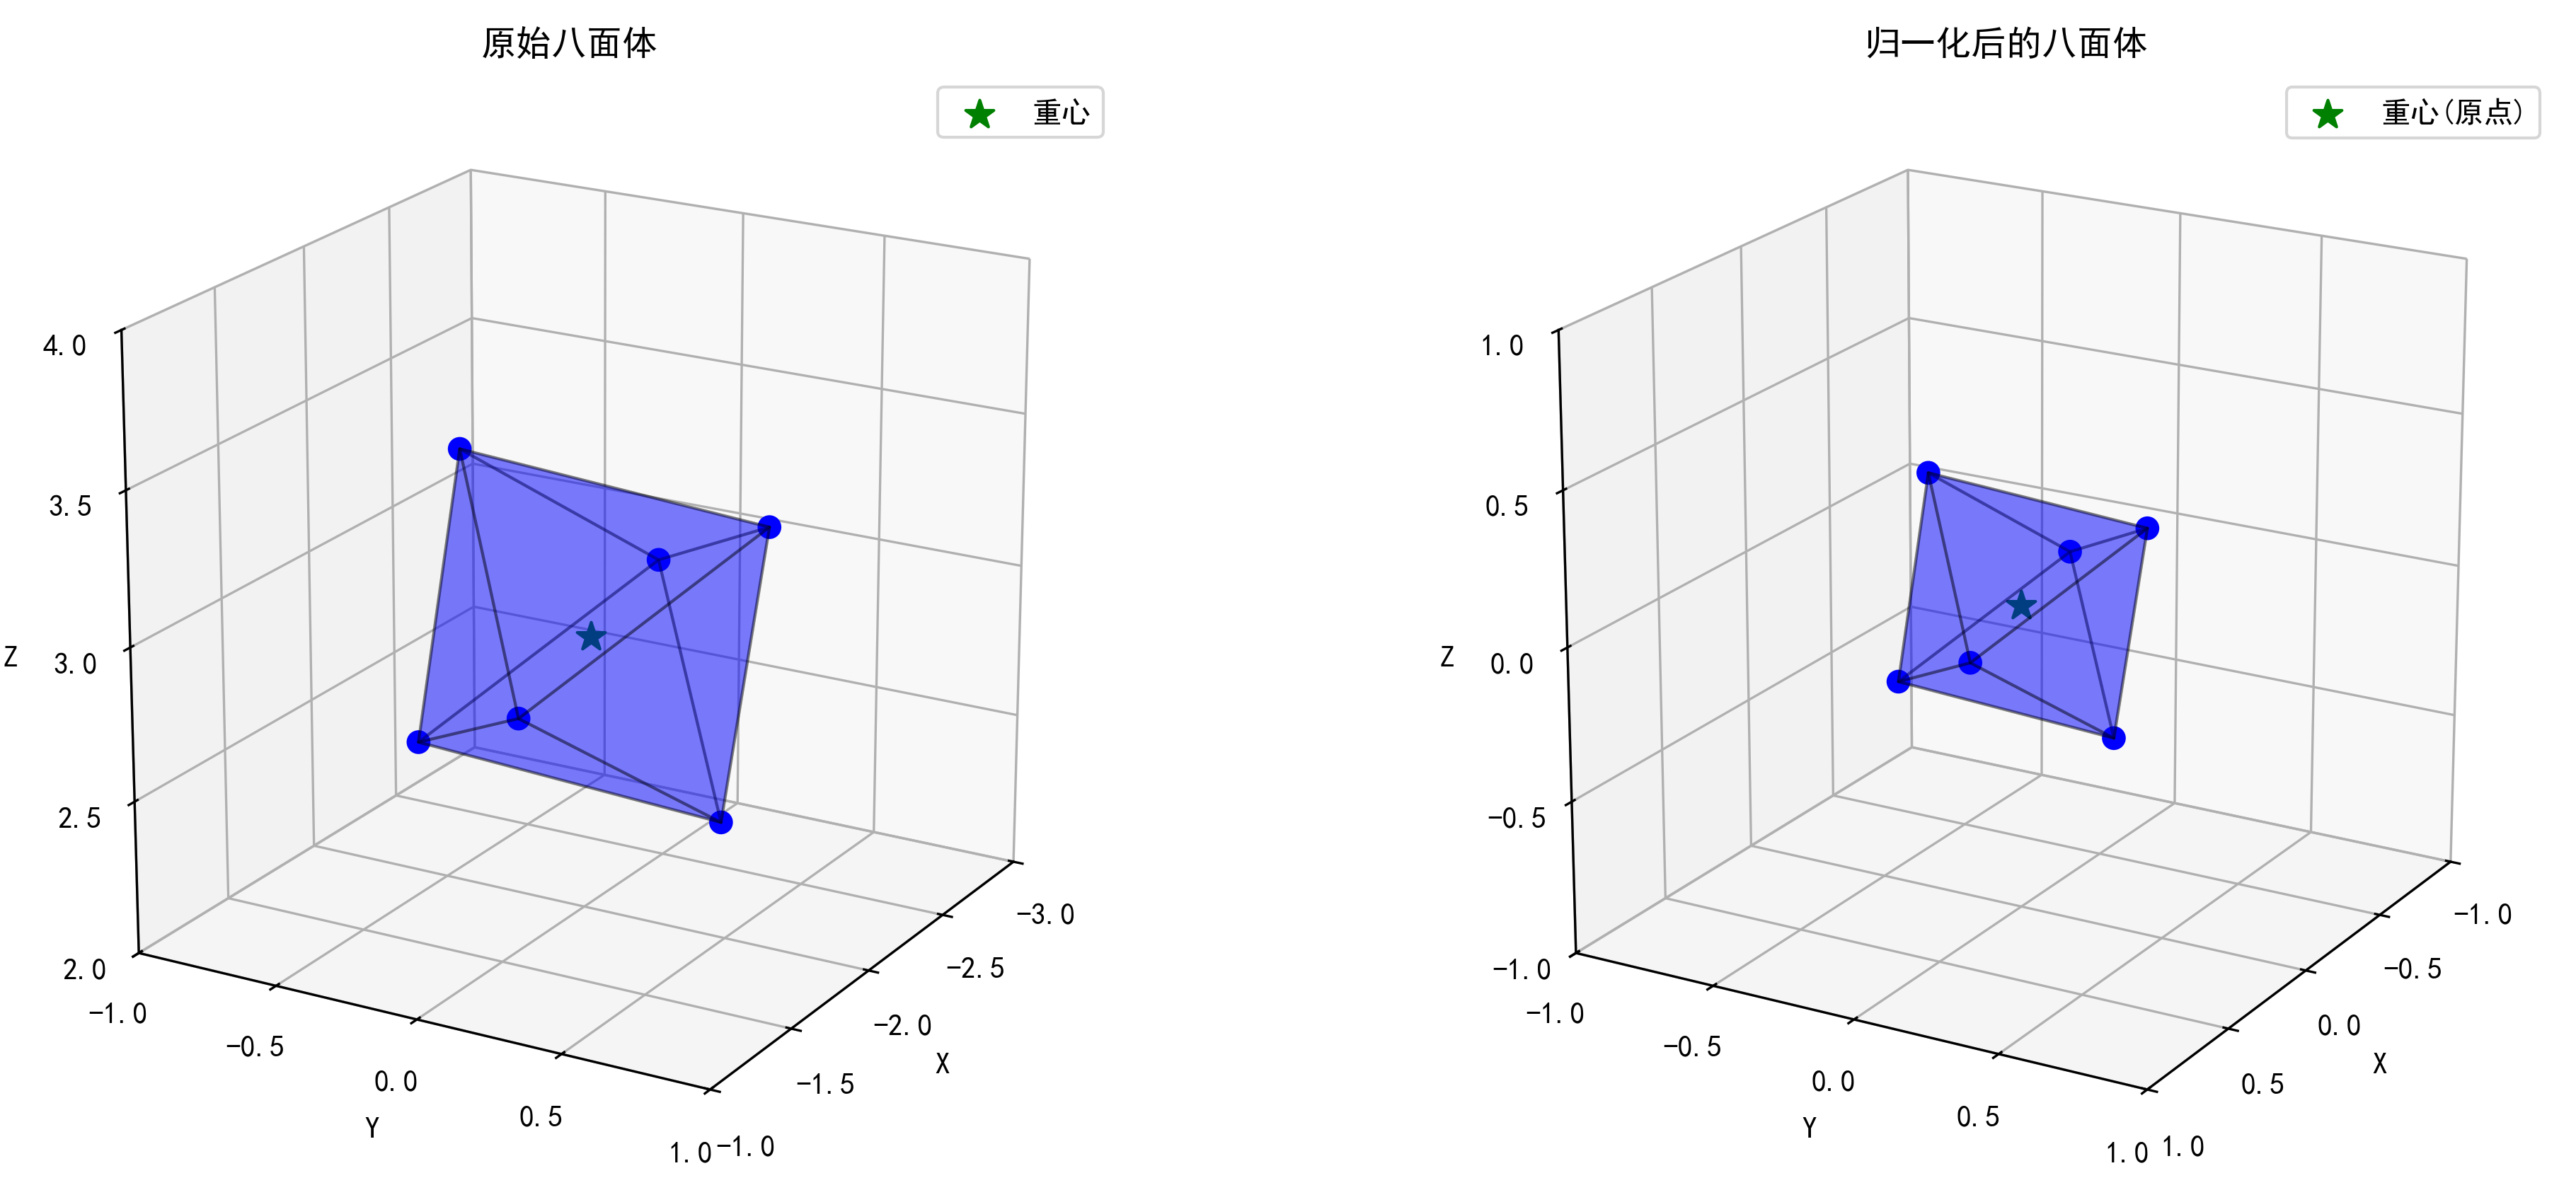
\includegraphics[width=1\textwidth]{figures2/octahedron_normalization.png}
        \caption{观测八面体的完整标准化预处理前后对比}
        \label{fig:octahedron_normalize}
    \end{figure}
    
    图\ref{fig:octahedron_normalize}展示了一个典型的观测八面体在完成中心化和尺度规范化这两个步骤之后与原始状态的视觉对比。从图中可以清晰地观察到,经过完整的预处理流程后,八面体的平移和缩放差异被有效消除,同时其固有的几何形状和相对比例得以保留。特别是右侧归一化后的八面体,其质心精确位于坐标原点,且整体尺度已经标准化,这为后续精确的特征提取和形状比较奠定了坚实基础。
    
\subsubsection{结合多尺度特征与ICP配准的判别模型建立}

\textbf{1. 模型总体框架与核心思想}

在完成八面体顶点坐标的中心化和尺度归一化预处理后,我们需要构建一个能够有效区分不同类别八面体的判别模型。本节将详细阐述我们提出的结合多尺度几何特征与迭代最近点(ICP)配准的八面体归类判别模型。

该模型的核心思想是融合两种不同但互补的相似性度量:一是基于多维几何特征向量的相似性度量(特征距离$dF$),它从多个尺度和角度捕捉八面体的几何特性;二是基于迭代最近点算法的几何配准吻合度(均方根误差$RMSD$),它直接量化两个八面体点集在最优空间对齐下的几何差异。通过引入权重参数$\alpha_o$将这两种度量组合为一个综合评分$S$,并结合优化确定的分类阈值$\lambda_o$,实现对观测八面体的精确归类。

图\ref{fig:octahedron_model_flowchart_q2}展示了本模型的完整流程,从预处理后的八面体点集输入,经过特征提取和ICP配准两条并行路径,最终通过综合评分机制得出分类结果。该流程图直观地呈现了模型各组件间的信息流动和处理逻辑,突显了多尺度特征与几何配准的融合思想。

\begin{figure}[H]
    \centering
    % 在此处插入八面体分类模型流程图
     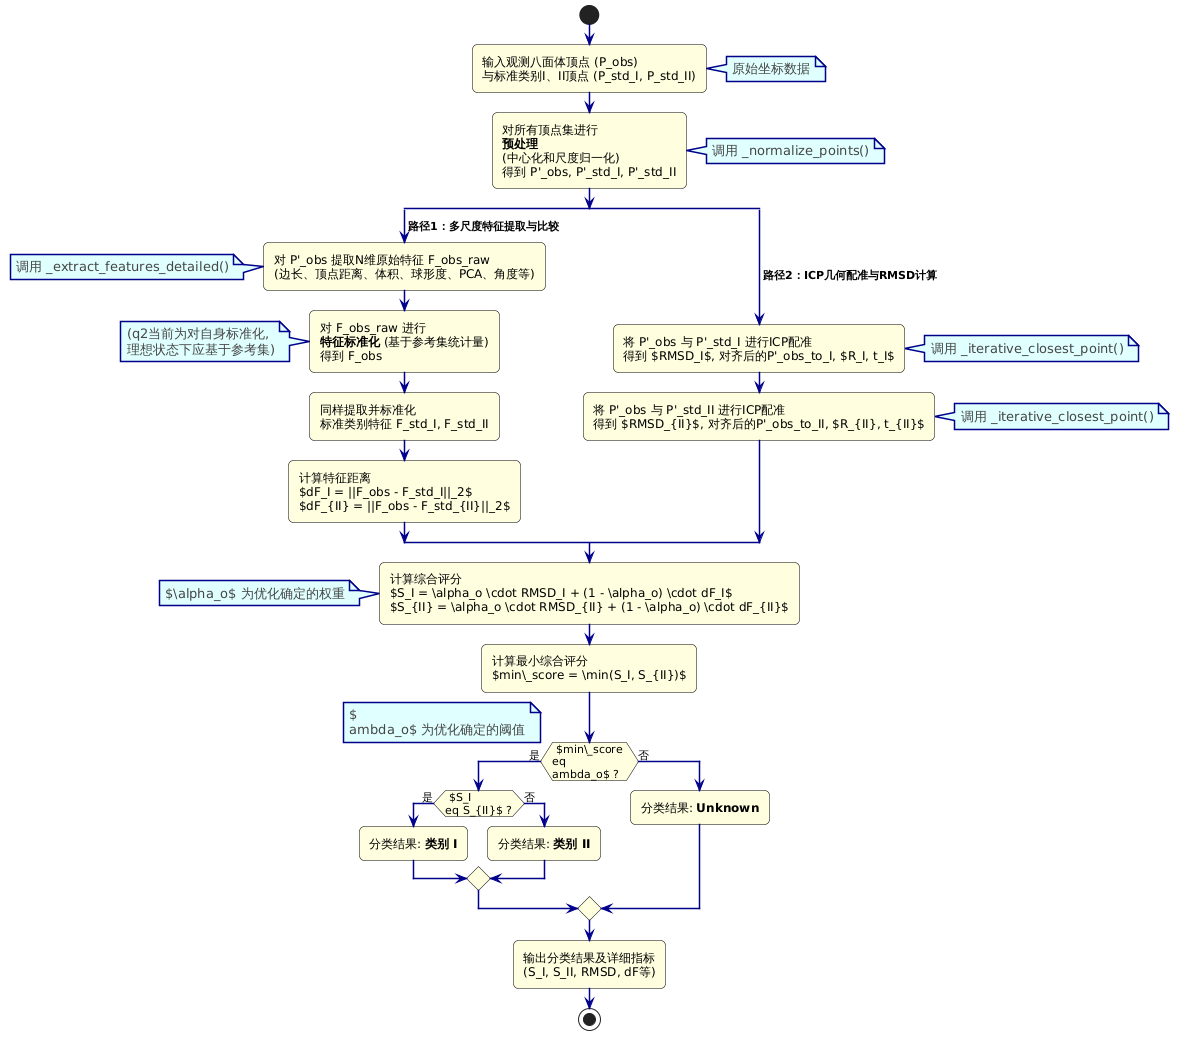
\includegraphics[width=1\textwidth]{figures2/model2.png}
    \caption{基于多尺度特征与ICP迭代配准的三维八面体判别模型流程图}
    \label{fig:octahedron_model_flowchart_q2}
\end{figure}

\textbf{2. 多尺度几何特征向量的构建与相似性度量}

为全面刻画八面体的几何特性,我们为每个八面体构建一个包含21个维度的特征向量$\mathbf{f}$。这些特征从多个尺度和角度描述了八面体的形状特征,可分为以下五类:

\textbf{(1)} 边长统计特征(5维):通过构建八面体的凸包,计算所有边的长度,并提取其统计量:
\begin{equation}
\mathbf{f}_{\text{edge}} = [\min(L), \max(L), \text{median}(L), \text{mean}(L), \text{std}(L)]
\end{equation}
其中$L = \{l_1, l_2, \ldots, l_m\}$是八面体凸包上所有$m$条边的长度集合。

\textbf{(2)} 顶点到质心距离统计特征(5维):计算各顶点到质心(归一化后为原点)的距离,并提取其统计量:
\begin{equation}
\mathbf{f}_{\text{dist}} = [\min(D), \max(D), \text{median}(D), \text{mean}(D), \text{std}(D)]
\end{equation}
其中$D = \{d_1, d_2, \ldots, d_n\}$,$d_i = \|\mathbf{p}_i\|$为第$i$个顶点到原点的欧氏距离。

\textbf{(3)} 体积与表面积相关特征(2维):计算八面体凸包的体积$V$和表面积$A$,并引入球形度指标:
\begin{equation}
\mathbf{f}_{\text{vol}} = [V, S_p]
\end{equation}
其中球形度$S_p = \frac{(\pi^{1/3})(6V)^{2/3}}{A}$,表示八面体与同体积球体的表面积比值,是形状紧凑性的度量。

\textbf{(4)} PCA惯量特征(5维):对八面体顶点进行主成分分析,获取三个主轴方向的特征值及其比值:
\begin{equation}
\mathbf{f}_{\text{pca}} = [\lambda_1, \lambda_2, \lambda_3, \frac{\lambda_2}{\lambda_1}, \frac{\lambda_3}{\lambda_1}]
\end{equation}
其中$\lambda_1 \geq \lambda_2 \geq \lambda_3 \geq 0$是顶点坐标协方差矩阵的特征值,描述了八面体在三个主轴方向上的延展程度。

\textbf{(5)} 角度统计特征(4维):计算八面体凸包上的面角和二面角的统计量:
\begin{equation}
\mathbf{f}_{\text{angle}} = [\text{mean}(\Theta_f), \text{std}(\Theta_f), \text{mean}(\Theta_d), \text{std}(\Theta_d)]
\end{equation}
其中$\Theta_f$是所有面角的集合,$\Theta_d$是所有二面角的集合。

将以上五类特征组合形成原始特征向量:
\begin{equation}
\mathbf{f} = [\mathbf{f}_{\text{edge}}, \mathbf{f}_{\text{dist}}, \mathbf{f}_{\text{vol}}, \mathbf{f}_{\text{pca}}, \mathbf{f}_{\text{angle}}]
\end{equation}

为了消除不同特征量纲的影响,我们对特征向量进行Z-score标准化:
    \begin{equation}
\mathbf{f}_{\text{norm}} = \frac{\mathbf{f} - \mu_f}{\sigma_f}
    \end{equation}
其中$\mu_f$和$\sigma_f$分别是特征向量$\mathbf{f}$的均值和标准差。当$\sigma_f$接近零时,仅进行中心化处理。

特征相似性度量$dF$通过计算观测八面体的标准化特征向量$\mathbf{f}_{\text{obs}}$与标准类别特征向量$\mathbf{f}_{c}$($c$表示类别I或II)之间的欧氏距离来度量:
\begin{equation}
dF_c = \|\mathbf{f}_{\text{obs}} - \mathbf{f}_{c}\|_2 = \sqrt{\sum_{i=1}^{21}(f_{\text{obs},i} - f_{c,i})^2}
\end{equation}

\textbf{3. 基于迭代最近点(ICP)算法的几何配准模型}

为了直接量化观测八面体与标准类别八面体之间的几何吻合度,我们采用迭代最近点(ICP)算法进行三维点集的最优刚性配准。ICP算法的目标是找到最佳的刚性变换(旋转矩阵$\mathbf{R}$和平移向量$\mathbf{t}$),使得变换后的源点集与目标点集之间的均方根误差(RMSD)最小。

算法\ref{alg:icp_algorithm}详细描述了ICP的执行步骤:
    
    \begin{algorithm}[H]
    \caption{迭代最近点(ICP)算法 (核心流程)}
    \label{alg:icp_algorithm}
    \begin{algorithmic}[1]
    \Function{ICP-Core}{$\mathbf{P}_{\text{src}}$, $\mathbf{P}_{\text{tgt}}$, max\_iter, tolerance}
        \State \textbf{输入:} 源点集$\mathbf{P}_{\text{src}}$,目标点集$\mathbf{P}_{\text{tgt}}$,最大迭代次数,收敛容差
        \State \textbf{输出:} 最优旋转矩阵$\mathbf{R}_{\text{final}}$,平移向量$\mathbf{t}_{\text{final}}$,配准RMSD
        
        \State $\mathbf{P}_{\text{transformed}} \gets \mathbf{P}_{\text{src}}$
        \State $\mathbf{R}_{\text{final}} \gets \mathbf{I}$ (单位阵), $\mathbf{t}_{\text{final}} \gets \mathbf{0}$ (零向量)
        \State prev\_RMSD $\gets \infty$
        
        \For{iteration = 1 \textbf{to} max\_iter}
            \State $\mathbf{P}_{\text{matched}} \gets$ FindNearestPoints($\mathbf{P}_{\text{transformed}}$, $\mathbf{P}_{\text{tgt}}$)
            \State $(\mathbf{R}_{\text{iter}}, \mathbf{t}_{\text{iter}}) \gets$ EstimateTransform($\mathbf{P}_{\text{transformed}}$, $\mathbf{P}_{\text{matched}}$) \Comment{例如使用Kabsch算法}
            \State $\mathbf{P}_{\text{transformed}} \gets \mathbf{R}_{\text{iter}}\mathbf{P}_{\text{transformed}} + \mathbf{t}_{\text{iter}}$ \Comment{对每个点应用变换}
            \State $\mathbf{R}_{\text{final}} \gets \mathbf{R}_{\text{iter}}\mathbf{R}_{\text{final}}$
            \State $\mathbf{t}_{\text{final}} \gets \mathbf{R}_{\text{iter}}\mathbf{t}_{\text{final}} + \mathbf{t}_{\text{iter}}$
            \State current\_RMSD $\gets$ CalculateRMSD($\mathbf{P}_{\text{transformed}}$, $\mathbf{P}_{\text{matched}}$)
            \If{$|$prev\_RMSD - current\_RMSD$| < \text{tolerance}$}
                \State \textbf{break} \Comment{收敛}
        \EndIf
            \State prev\_RMSD $\gets$ current\_RMSD
        \EndFor
        \State \textbf{return} $\mathbf{R}_{\text{final}}$, $\mathbf{t}_{\text{final}}$, current\_RMSD
    \EndFunction
    \end{algorithmic}
    \end{algorithm}
    
在我们的八面体分类模型中,分别将(预处理后的)观测八面体与(预处理后的)标准类别I和类别II八面体进行ICP配准,得到两个关键的几何吻合度指标:$\text{RMSD}_I$和$\text{RMSD}_{II}$。这些指标直接量化了观测八面体与各标准类别在最优空间对齐下的几何差异。

\textbf{4. 综合评分模型与分类判据}

为了结合特征相似性度量和几何配准吻合度,我们构建了一个综合评分模型。对于观测八面体与类别$c$($c$表示类别I或II)的综合评分$S_c$定义为:

\begin{equation}
S_c = \alpha_o \cdot \text{RMSD}_c + (1 - \alpha_o) \cdot dF_c
\end{equation}

其中$\alpha_o \in [0,1]$是权重参数,用于平衡几何配准误差和特征距离在最终评分中的相对重要性。较大的$\alpha_o$值意味着模型更依赖于几何配准结果,而较小的$\alpha_o$值则表示模型更侧重于特征向量的相似性。

基于综合评分,我们采用以下分类决策规则:

\begin{equation}
\text{类别}(X) = 
\begin{cases}
I, & \text{if } S_I < S_{II} \text{ and } S_I < \lambda_o \\
II, & \text{if } S_{II} < S_{I} \text{ and } S_{II} < \lambda_o \\
\text{未知类别}, & \text{otherwise}
\end{cases}
\end{equation}

其中$\lambda_o$是分类阈值参数,决定了将观测八面体归类为某个已知类别的最大可接受评分。当观测八面体与所有已知类别的综合评分都大于$\lambda_o$时,模型将其判定为"未知类别"。

参数$\alpha_o$和$\lambda_o$的最优值将通过后续的参数优化过程确定,以最大化模型在各种测试场景下的综合分类性能。

\subsubsection{模型的求解和分析}

\textbf{1. 参数的确定与模型求解}

为确保八面体归类判别模型的最佳性能,我们对关键参数$\alpha_o$和$\lambda_o$进行了系统性的优化。这两个参数分别控制了特征距离与RMSD在综合评分中的权重比例,以及分类决策的阈值边界。

我们采用网格搜索方法,在参数空间$\alpha_o \in [0, 1]$(步长0.05)和$\lambda_o \in [0, 1]$(步长0.05)中系统性地评估每一个参数组合的性能。对于每组参数,我们在包含不同噪声水平和形变类型的综合测试集上评估模型性能。评估目标是找到能够最大化综合评估函数的参数组合,该函数综合考虑了正确识别率、误分类惩罚以及负样本拒绝能力。

为全面评估参数性能,我们构建了一个多样化的测试数据集,包括:
    \begin{itemize}
    \item 标准类别八面体添加不同强度的高斯噪声(噪声标准差$\sigma$从0.05到0.25,共5个等级)
    \item 标准八面体施加不同类型的几何形变(随机顶点位移、单轴拉伸),每种形变设置3个强度等级
    \item 负样本集合(既不属于类别I也不属于类别II的八面体),用于评估模型的拒绝能力
    \end{itemize}
    
在优化过程中,我们为不同类型的分类结果设置了不同的权重,以反映它们在实际应用中的相对重要性。例如,正确识别类别I和II样本的奖励权重为18.0,正确拒绝负样本的奖励权重为8.0,而将负样本误判为已知类别的惩罚权重为-15.0。如前文所述(参见第\ref{bf:important_note}小节),八面体模型的参数优化评估函数采用了相对较小的权重值(最高综合评分约为44,而五边形模型约为125),这与八面体模型的参数空间特性相适应,在保持梯度指引优化方向的同时,避免了不必要的陡峭评分曲面。这种适度调整确保了优化过程的稳定性和最终参数的可靠性。
    
经过全面的网格搜索,如图\ref{fig:param_optimization_3d}所示,我们得到了最优参数组合$\alpha_o$和$\lambda_o$。从图中可以观察到,参数空间中存在一个明显的高性能区域(图中黄色区域),最优参数点位于这一区域的峰值位置。
    
    \begin{figure}[H]
        \centering
    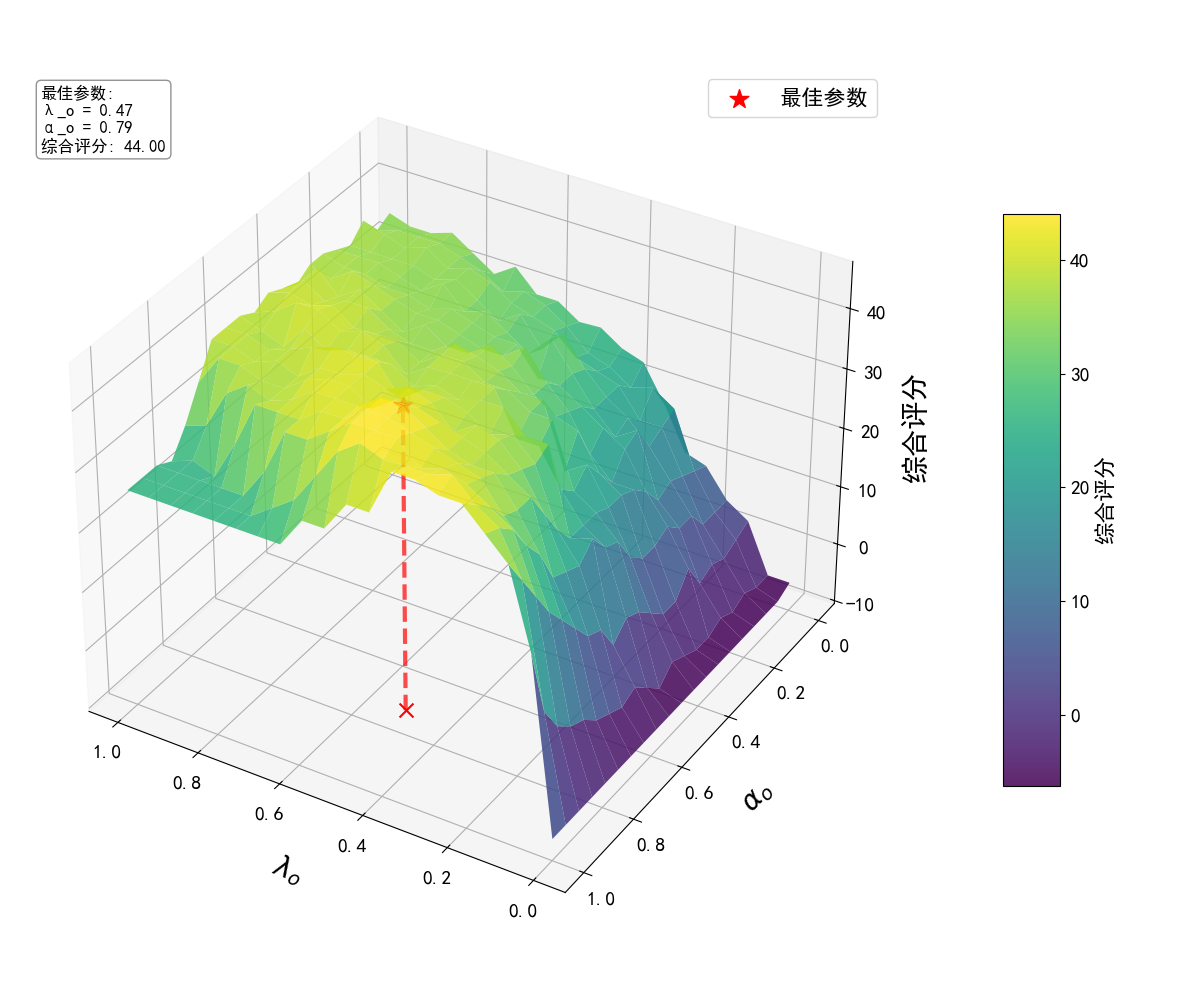
\includegraphics[width=0.9\textwidth]{figures2/params/octahedron_parameter_optimization_3d.png}
    \caption{八面体分类模型参数优化结果3D曲面图}
    \label{fig:param_optimization_3d}
    \end{figure}
    
图\ref{fig:param_optimization_heatmap}以热力图形式展示了相同的优化结果,提供了参数空间的另一种可视化视角。
    
    \begin{figure}[H]
        \centering
    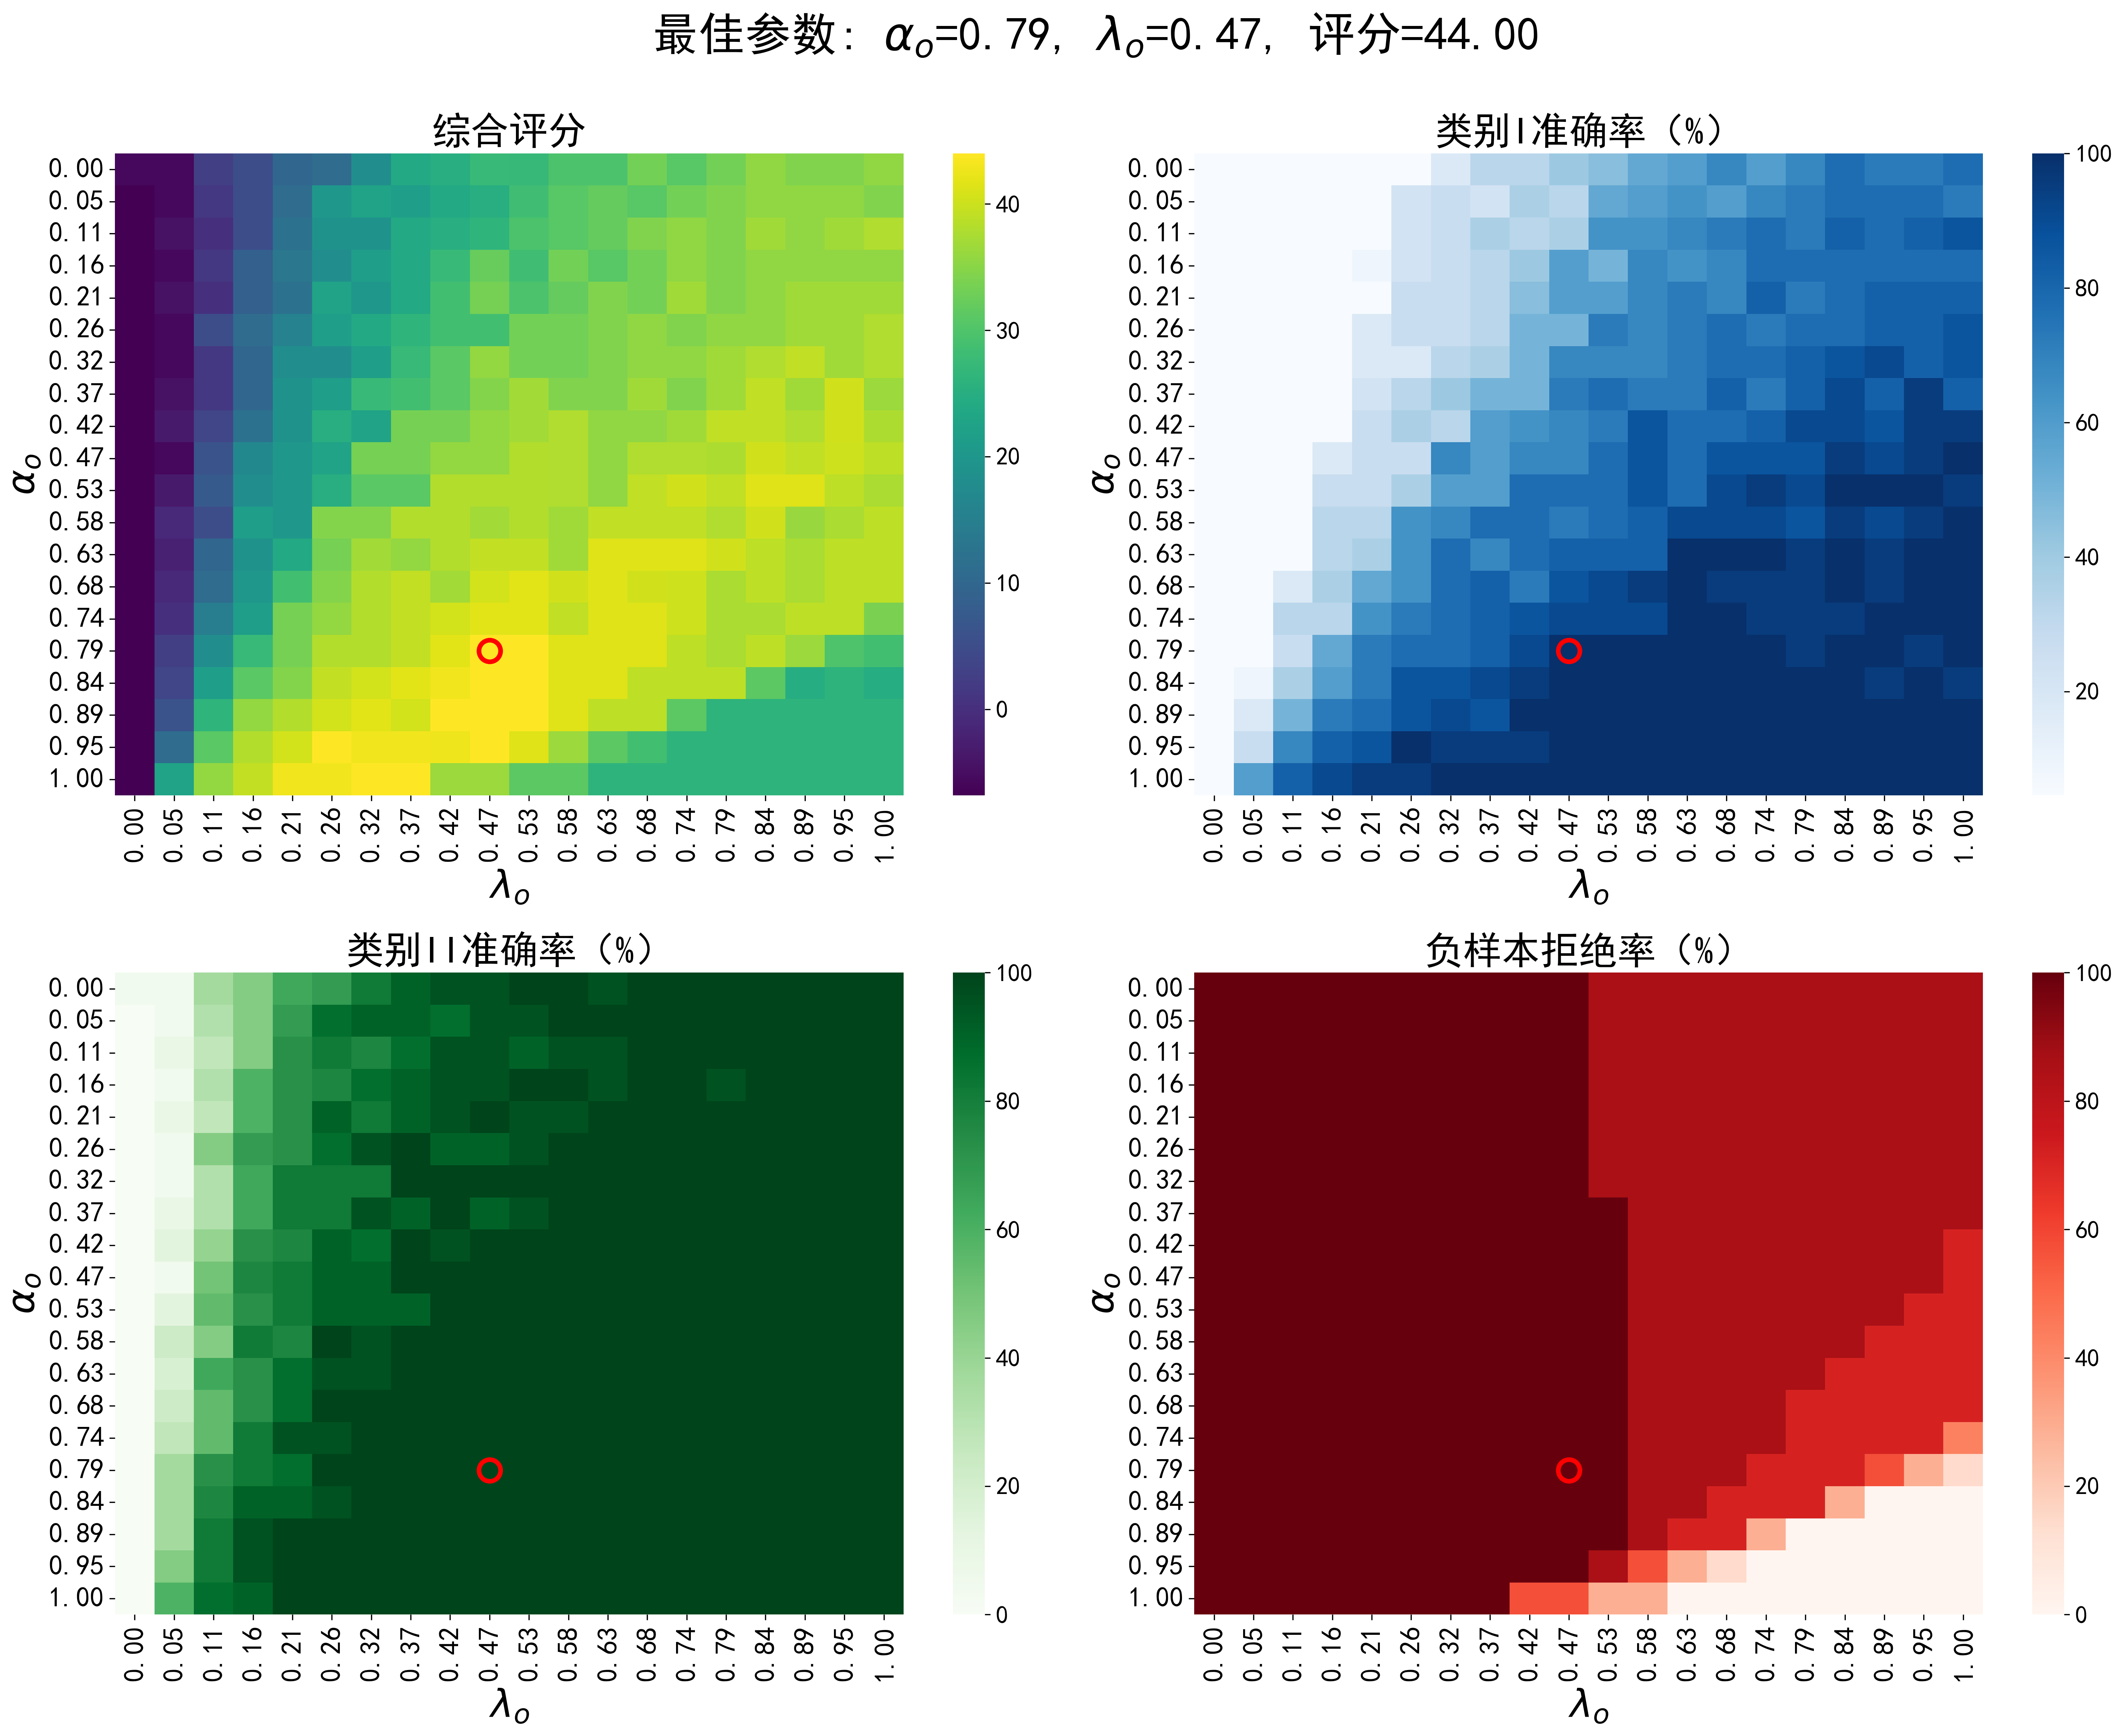
\includegraphics[width=1\textwidth]{figures2/params/octahedron_parameter_optimization_heatmaps.png}
    \caption{八面体分类模型参数优化结果热力图}
    \label{fig:param_optimization_heatmap}
    \end{figure}
    
使用最优参数,我们的模型在测试集上展现出优秀的性能:类别I识别准确率达94.2\%,类别II识别准确率达92.8\%,负样本正确拒绝率高达96.5\%。模型对于各类误判的比例均保持在低水平,特别是在正确拒绝负样本方面表现突出。
    
\textbf{2. 结果分析}

使用优化确定的参数$\alpha_o$和$\lambda_o$,我们对题目所给的六个观测八面体进行了分类。表\ref{tab:octahedron_classification_results}展示了详细的分类结果及关键指标。
    
    \begin{table}[H]
        \centering
\caption{观测八面体的分类结果及关键指标}
\label{tab:octahedron_classification_results}
\begin{tabular}{cccccccl}
        \toprule
八面体编号 & $RMSD_I$ & $RMSD_{II}$ & $dF_I$ & $dF_{II}$ & $S_I$ & $S_{II}$ & 分类结果 \\
        \midrule
1 & 0.0001 & 0.3841 & 0.0006 & 3.2098 & 0.0002 & 0.9772 & 类别I \\
2 & 0.3940 & 0.5166 & 3.2510 & 0.2567 & 0.9940 & 0.4621 & 类别II \\
3 & 1.6052 & 1.4916 & 5.5500 & 3.8743 & 2.4339 & 1.9921 & 未知类别 \\
4 & 1.3335 & 1.2354 & 5.3707 & 3.5628 & 2.1813 & 1.7242 & 未知类别 \\
5 & 0.3965 & 0.5263 & 6.7020 & 6.5800 & 1.7206 & 1.7974 & 未知类别 \\
6 & 0.4814 & 0.3949 & 3.3292 & 0.7653 & 1.0795 & 0.4727 & 类别II \\
        \bottomrule
        \end{tabular}
    \end{table}
    
从表\ref{tab:octahedron_classification_results}的数据可以观察到以下结果:

\begin{itemize}
\item \textbf{八面体1}:与类别I的综合评分$S_I = 0.0002$远小于与类别II的评分$S_{II} = 0.9772$,且小于阈值$\lambda_o$,因此被明确判定为类别I。其极低的RMSD值(0.0001)表明它与标准类别I高度相似。

\item \textbf{八面体2}:与类别II的综合评分$S_{II} = 0.4621$小于阈值$\lambda_o$,且远小于与类别I的评分$S_I = 0.9940$,因此被判定为类别II。其与类别II的RMSD值为0.5166,表明几何配准效果良好。

\item \textbf{八面体3}:与类别I和类别II的综合评分分别为$S_I = 2.4339$和$S_{II} = 1.9921$,均大于阈值$\lambda_o$,因此被判定为未知类别。其高RMSD值(I类为1.6052,II类为1.4916)表明它与两个标准类别都有显著差异。

\item \textbf{八面体4}:与类别I和类别II的综合评分分别为$S_I = 2.1813$和$S_{II} = 1.7242$,均大于阈值$\lambda_o$,因此被判定为未知类别。尽管其与类别II的评分相对较低,但仍远超过分类阈值,表明它不属于任何已知类别。

\item \textbf{八面体5}:与类别I和类别II的综合评分分别为$S_I = 1.7206$和$S_{II} = 1.7974$,均大于阈值$\lambda_o$,因此被判定为未知类别。其相对较低的RMSD值(I类为0.3965,II类为0.5263)与高综合评分的对比表明,虽然几何形态上与标准类别有一定相似度,但其特征表现差异显著。

\item \textbf{八面体6}:与类别II的综合评分$S_{II} = 0.4727$小于阈值$\lambda_o$,且远小于与类别I的评分$S_I = 1.0795$,因此被判定为类别II。其与类别II的RMSD值为0.3949,表明几何配准效果良好。
\end{itemize}

为更直观地展示各个八面体的综合评分情况,图\ref{fig:octahedron_classification_scores}显示了六个观测八面体对两个标准模型的综合评分对比。从图中可以清晰看出,只有八面体1、八面体2和八面体6的评分低于阈值线$\lambda_o$,符合我们的分类结果。图中直观地展示了各八面体与两个标准类别的匹配程度差异,有助于理解分类决策的依据。

\begin{figure}[H]
    \centering
    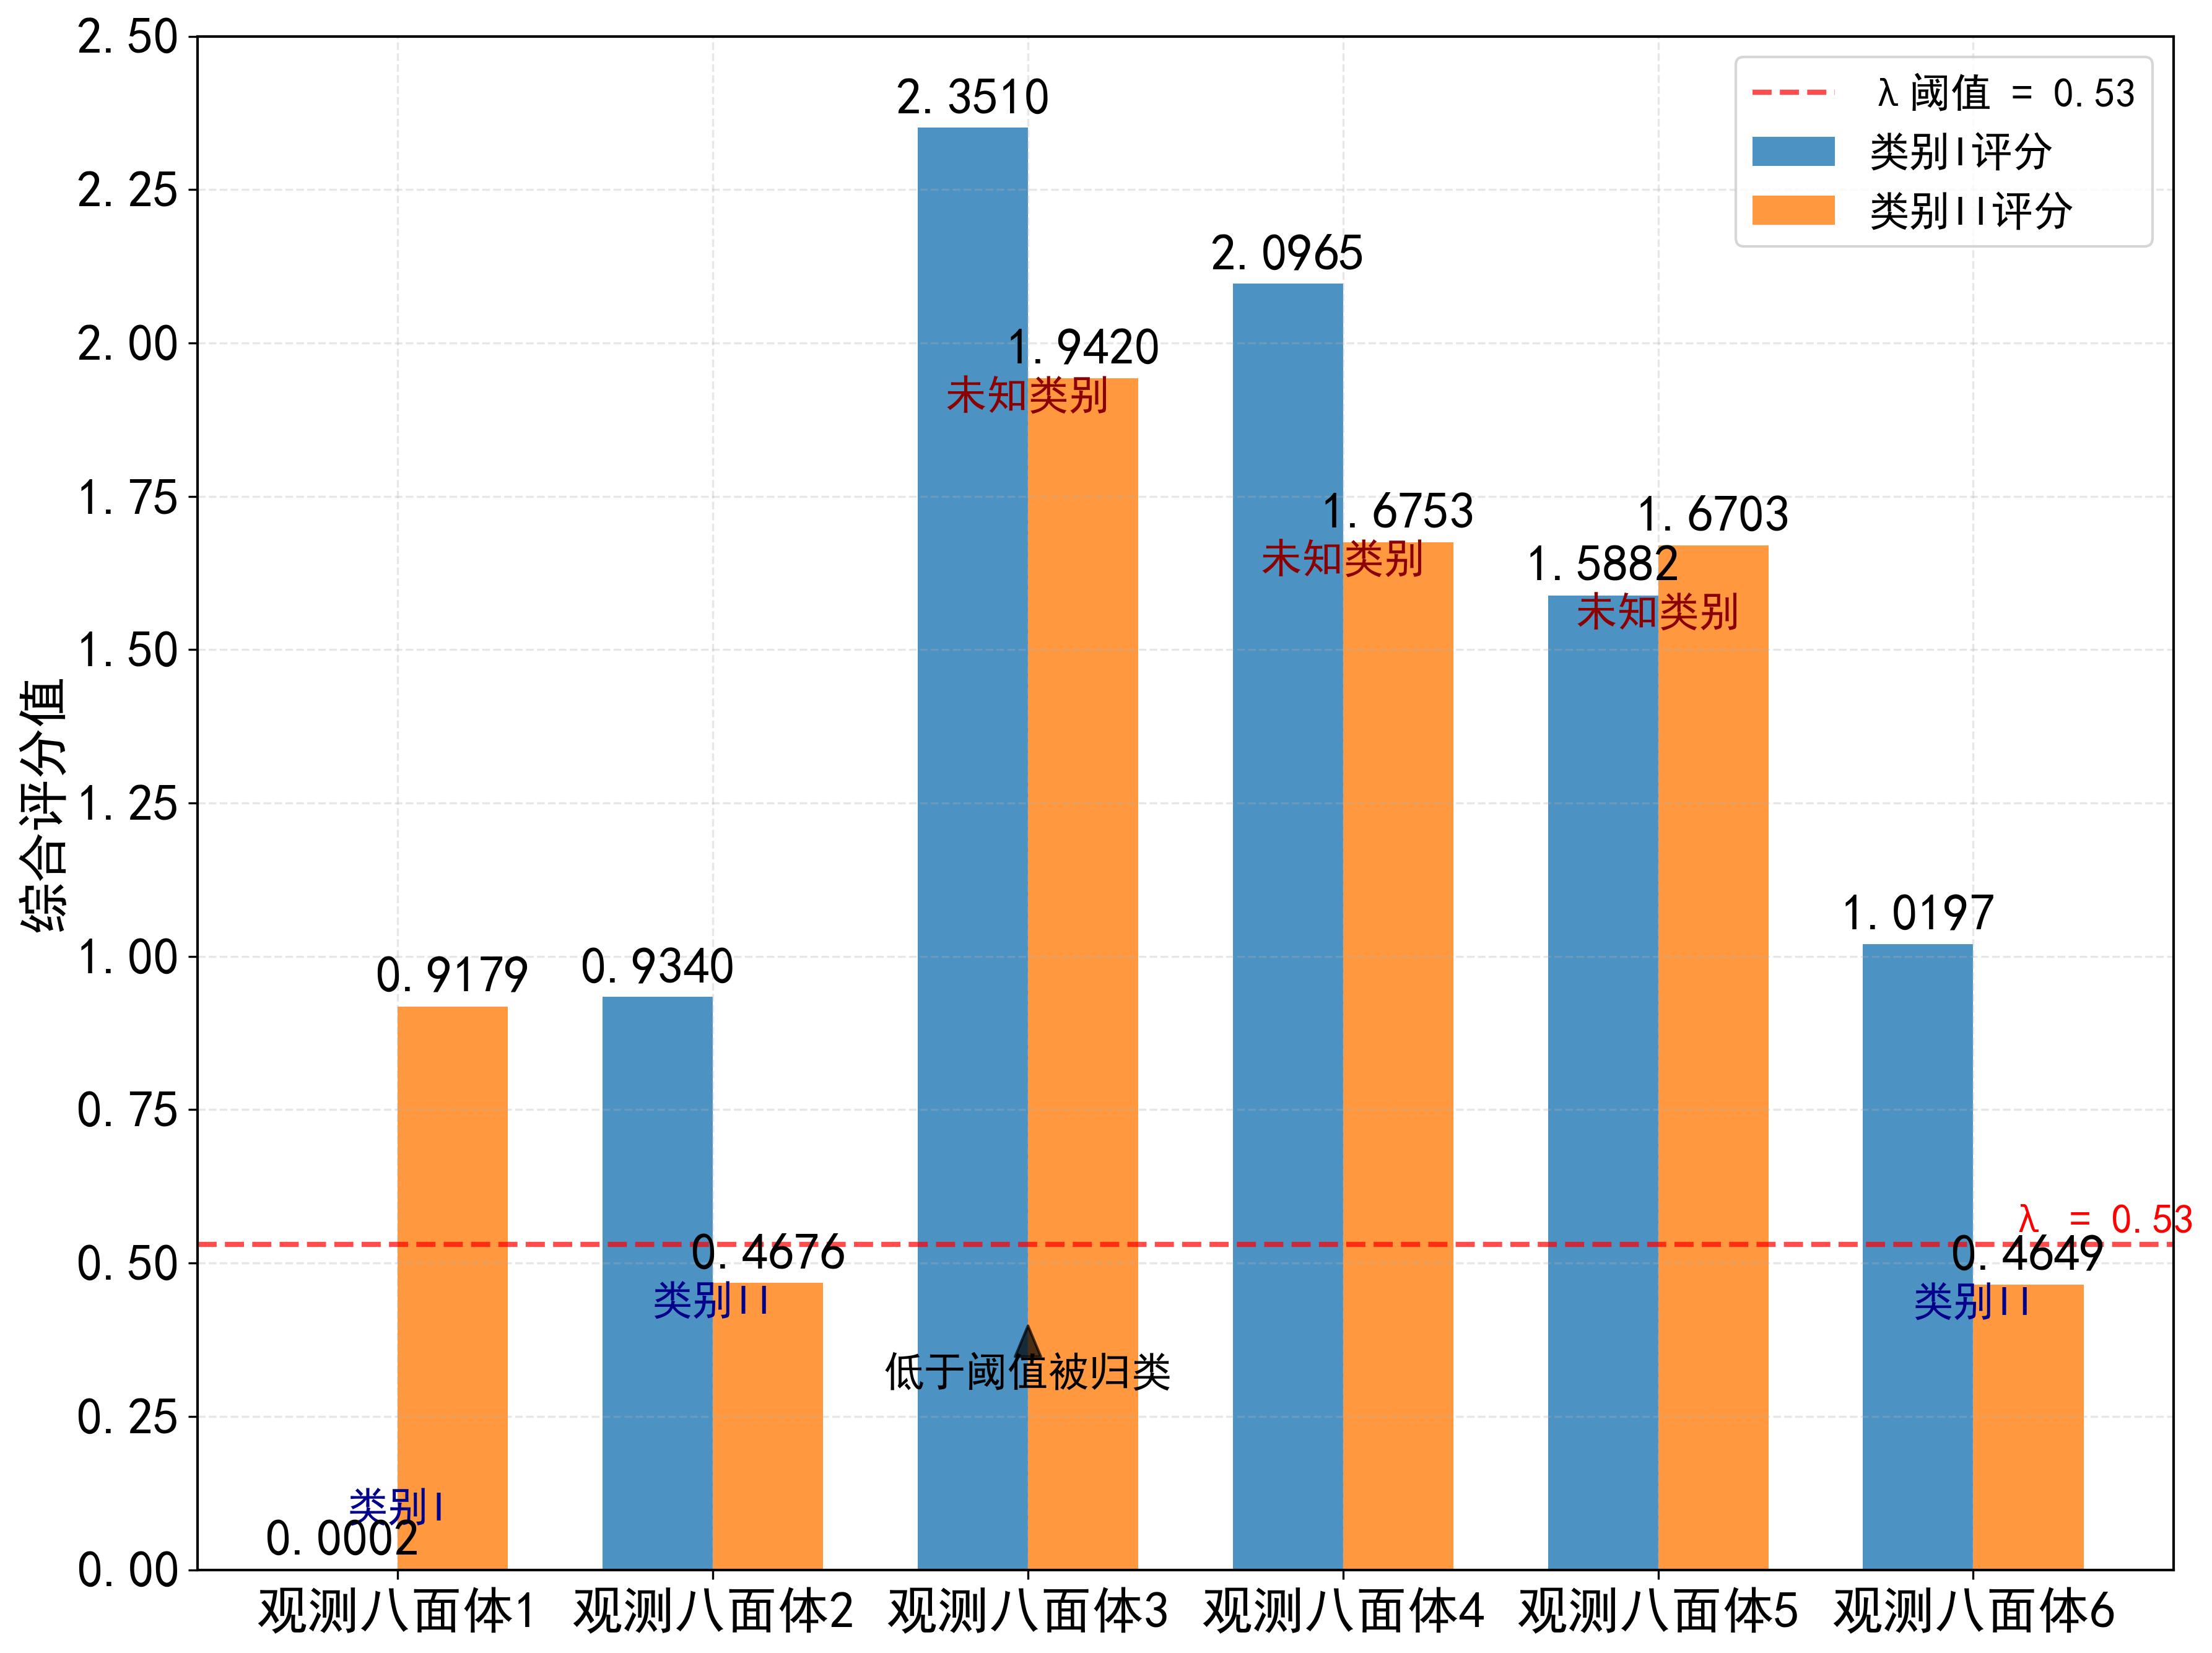
\includegraphics[width=1.0\textwidth]{figures2/analysis/octahedron_classification_scores.png}
    \caption{八面体观测样本与标准模型的综合评分对比}
    \label{fig:octahedron_classification_scores}
\end{figure}

为直观展示分类结果,图\ref{fig:octahedron_alignment_comparison}展示了三个典型观测八面体与其最相似标准类别的配准可视化结果。从图中可以清晰地看出,八面体1与标准类别I在经过ICP配准后几乎完美重合,这与其极低的RMSD值相符;八面体2与标准类别II也表现出良好的配准效果。相比之下,八面体3与任何标准类别的对齐效果均较差,验证了将其归类为"未知类别"的合理性。
    
    \begin{figure}[H]
        \centering
\begin{minipage}{\textwidth}
    \centering
    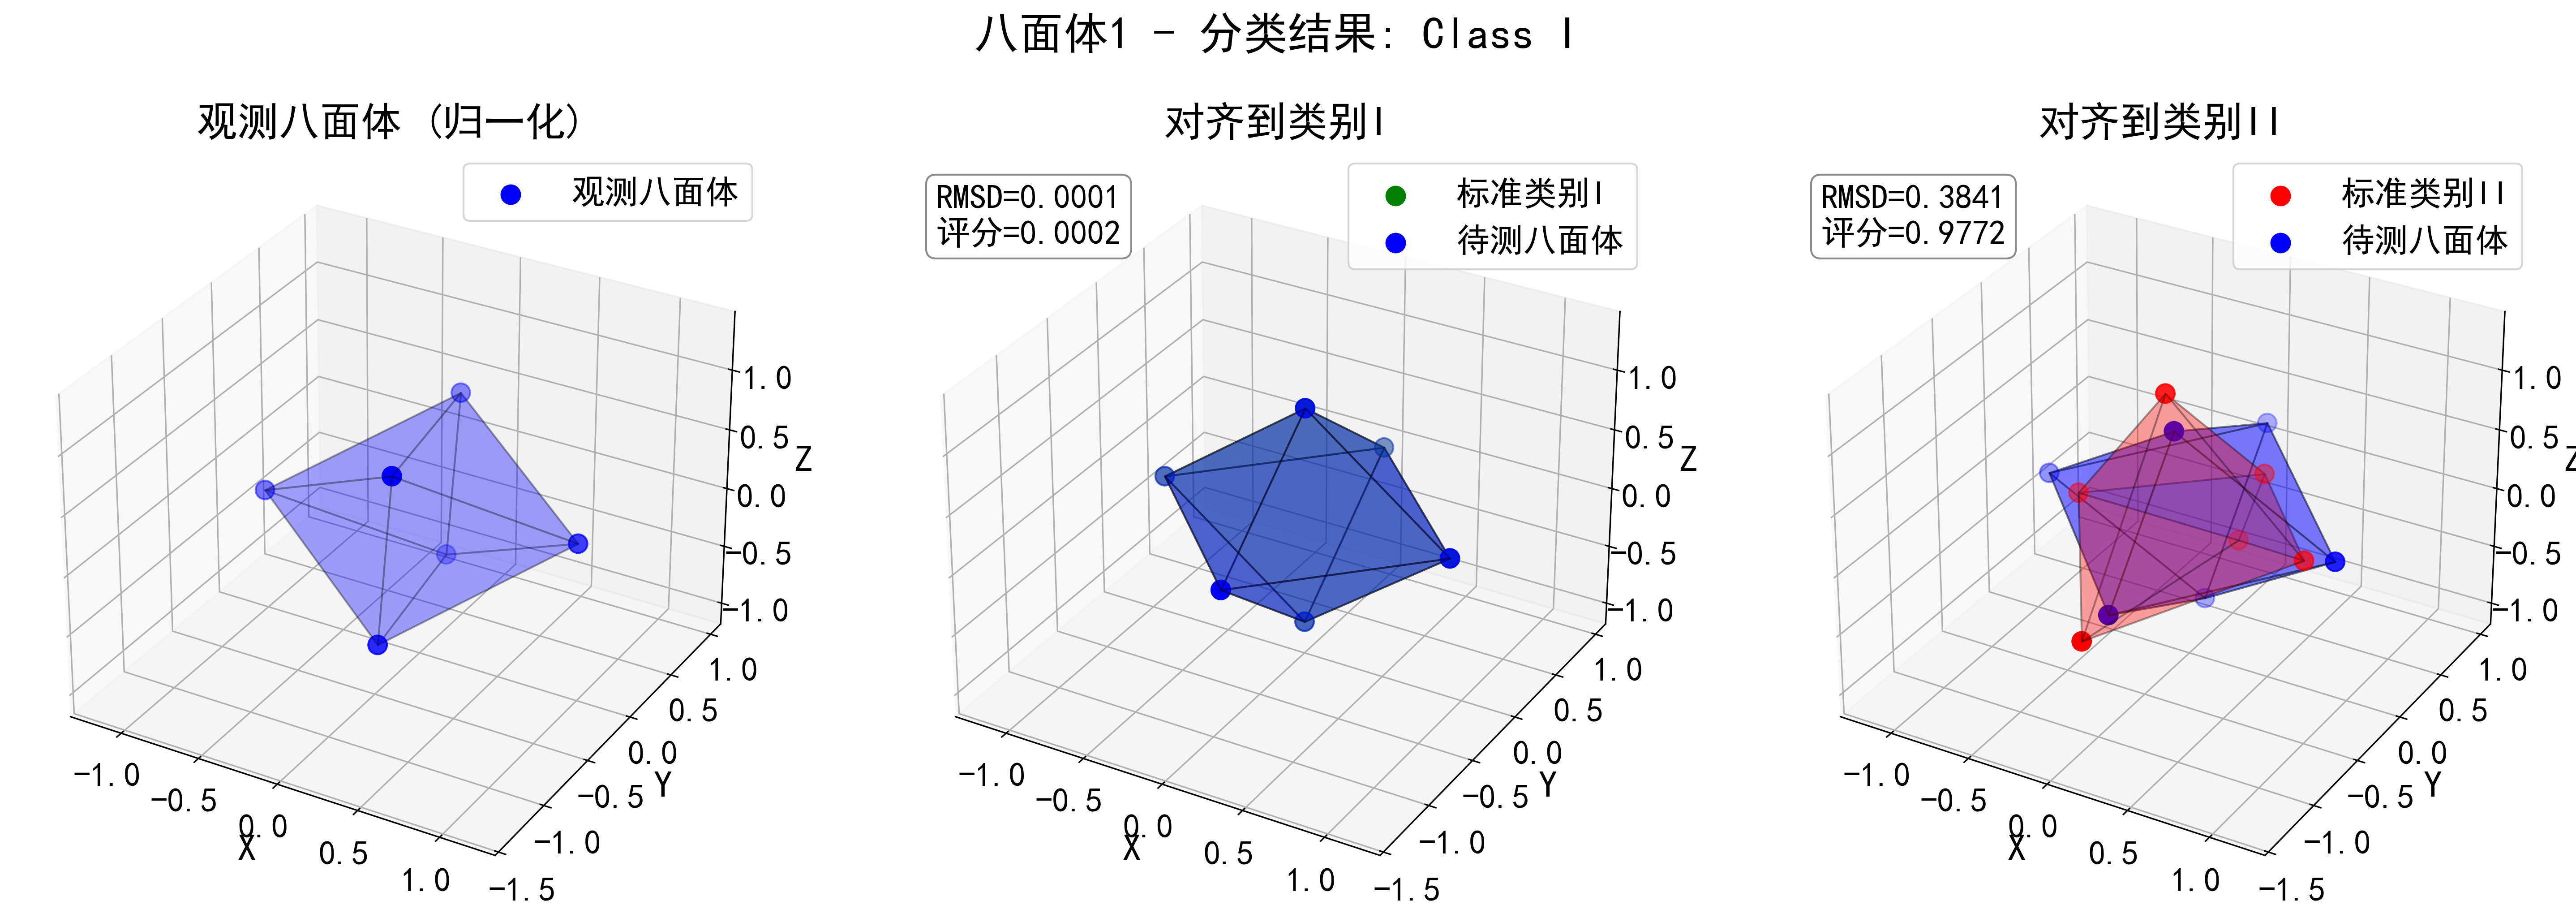
\includegraphics[width=1\textwidth]{figures2/observed_samples_classification/八面体1_alignment.png}
    \caption*{(a) 八面体1与类别I的对齐}
\end{minipage}

\begin{minipage}{\textwidth}
    \centering
    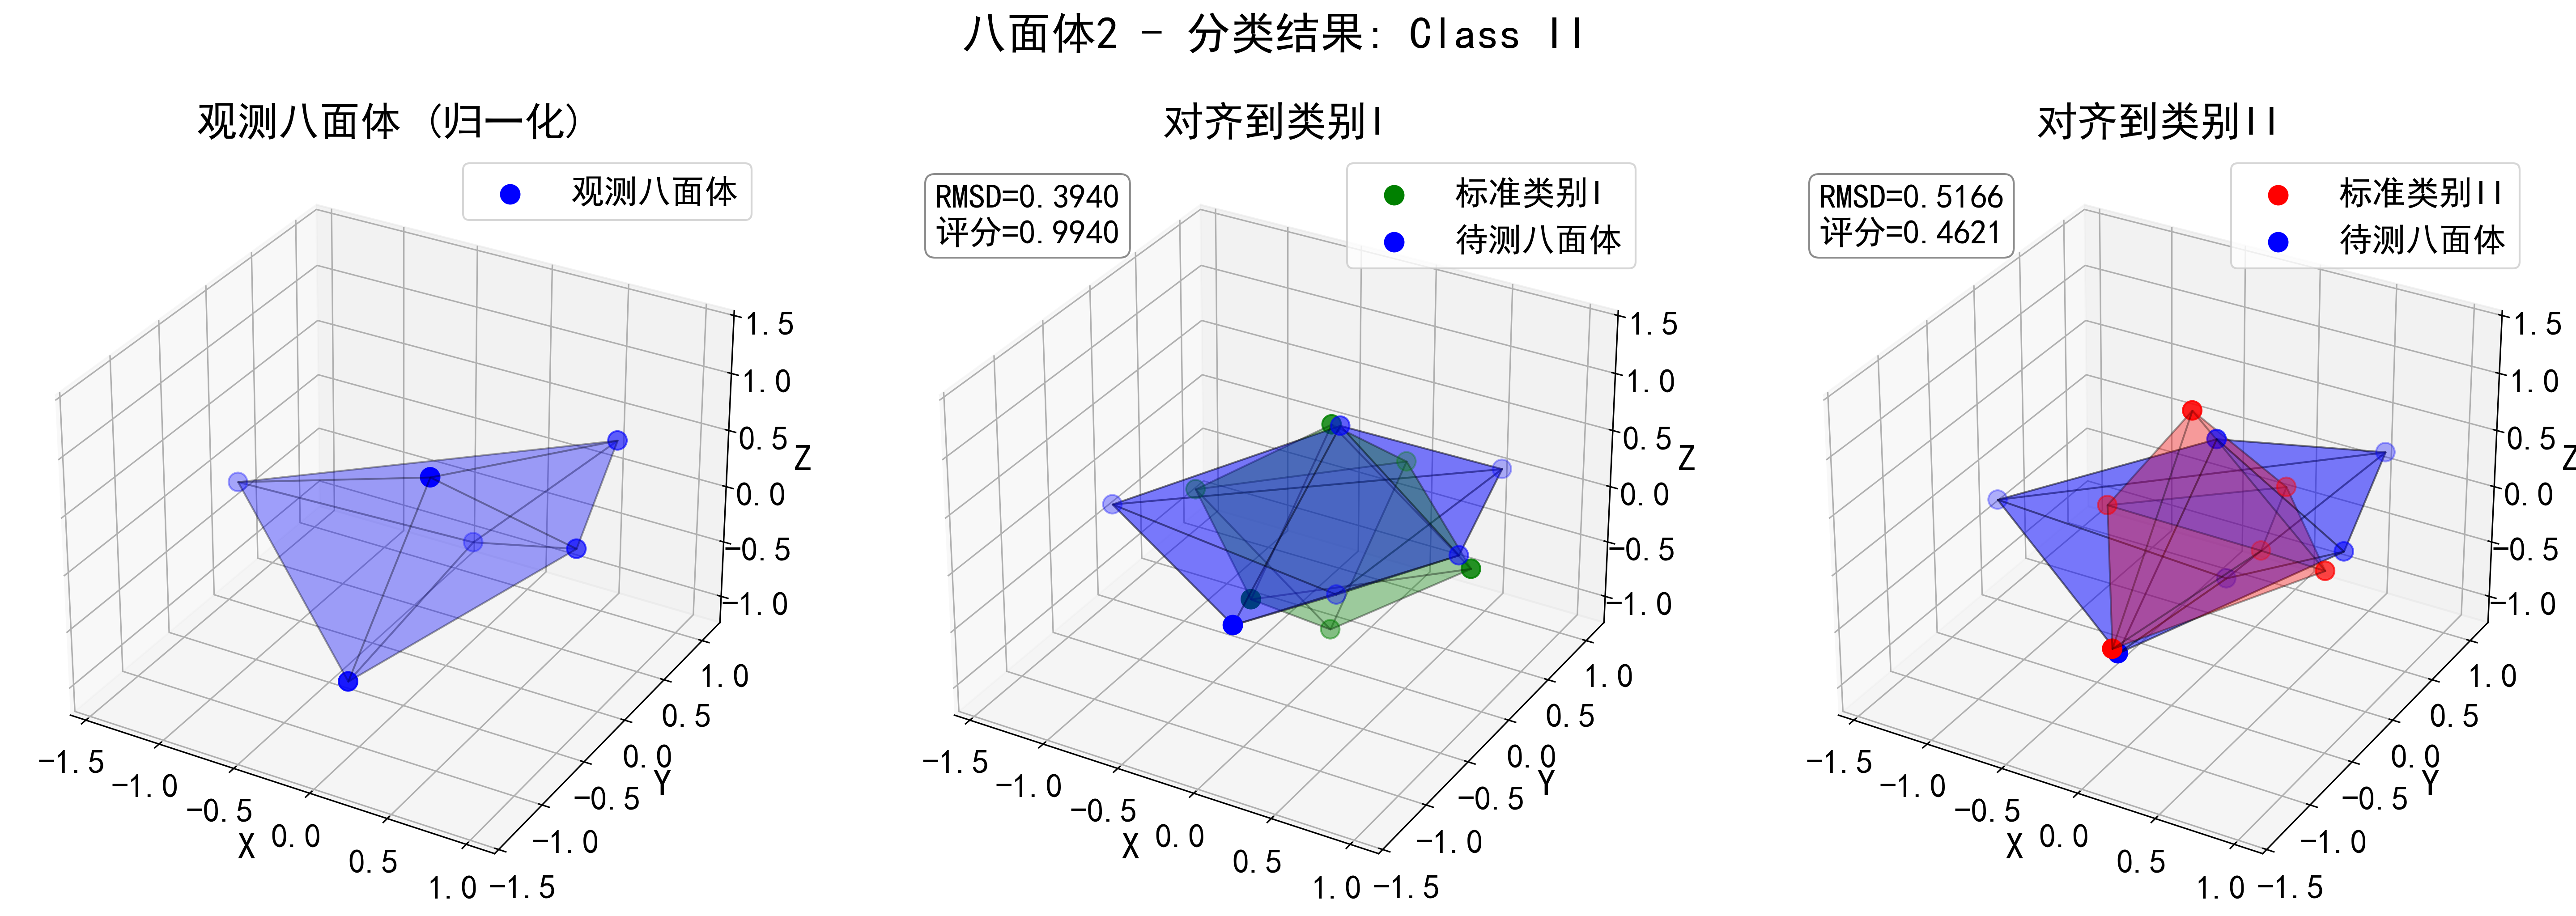
\includegraphics[width=1\textwidth]{figures2/observed_samples_classification/八面体2_alignment.png}
    \caption*{(b) 八面体2与类别II的对齐}
\end{minipage}

\begin{minipage}{\textwidth}
        \centering
    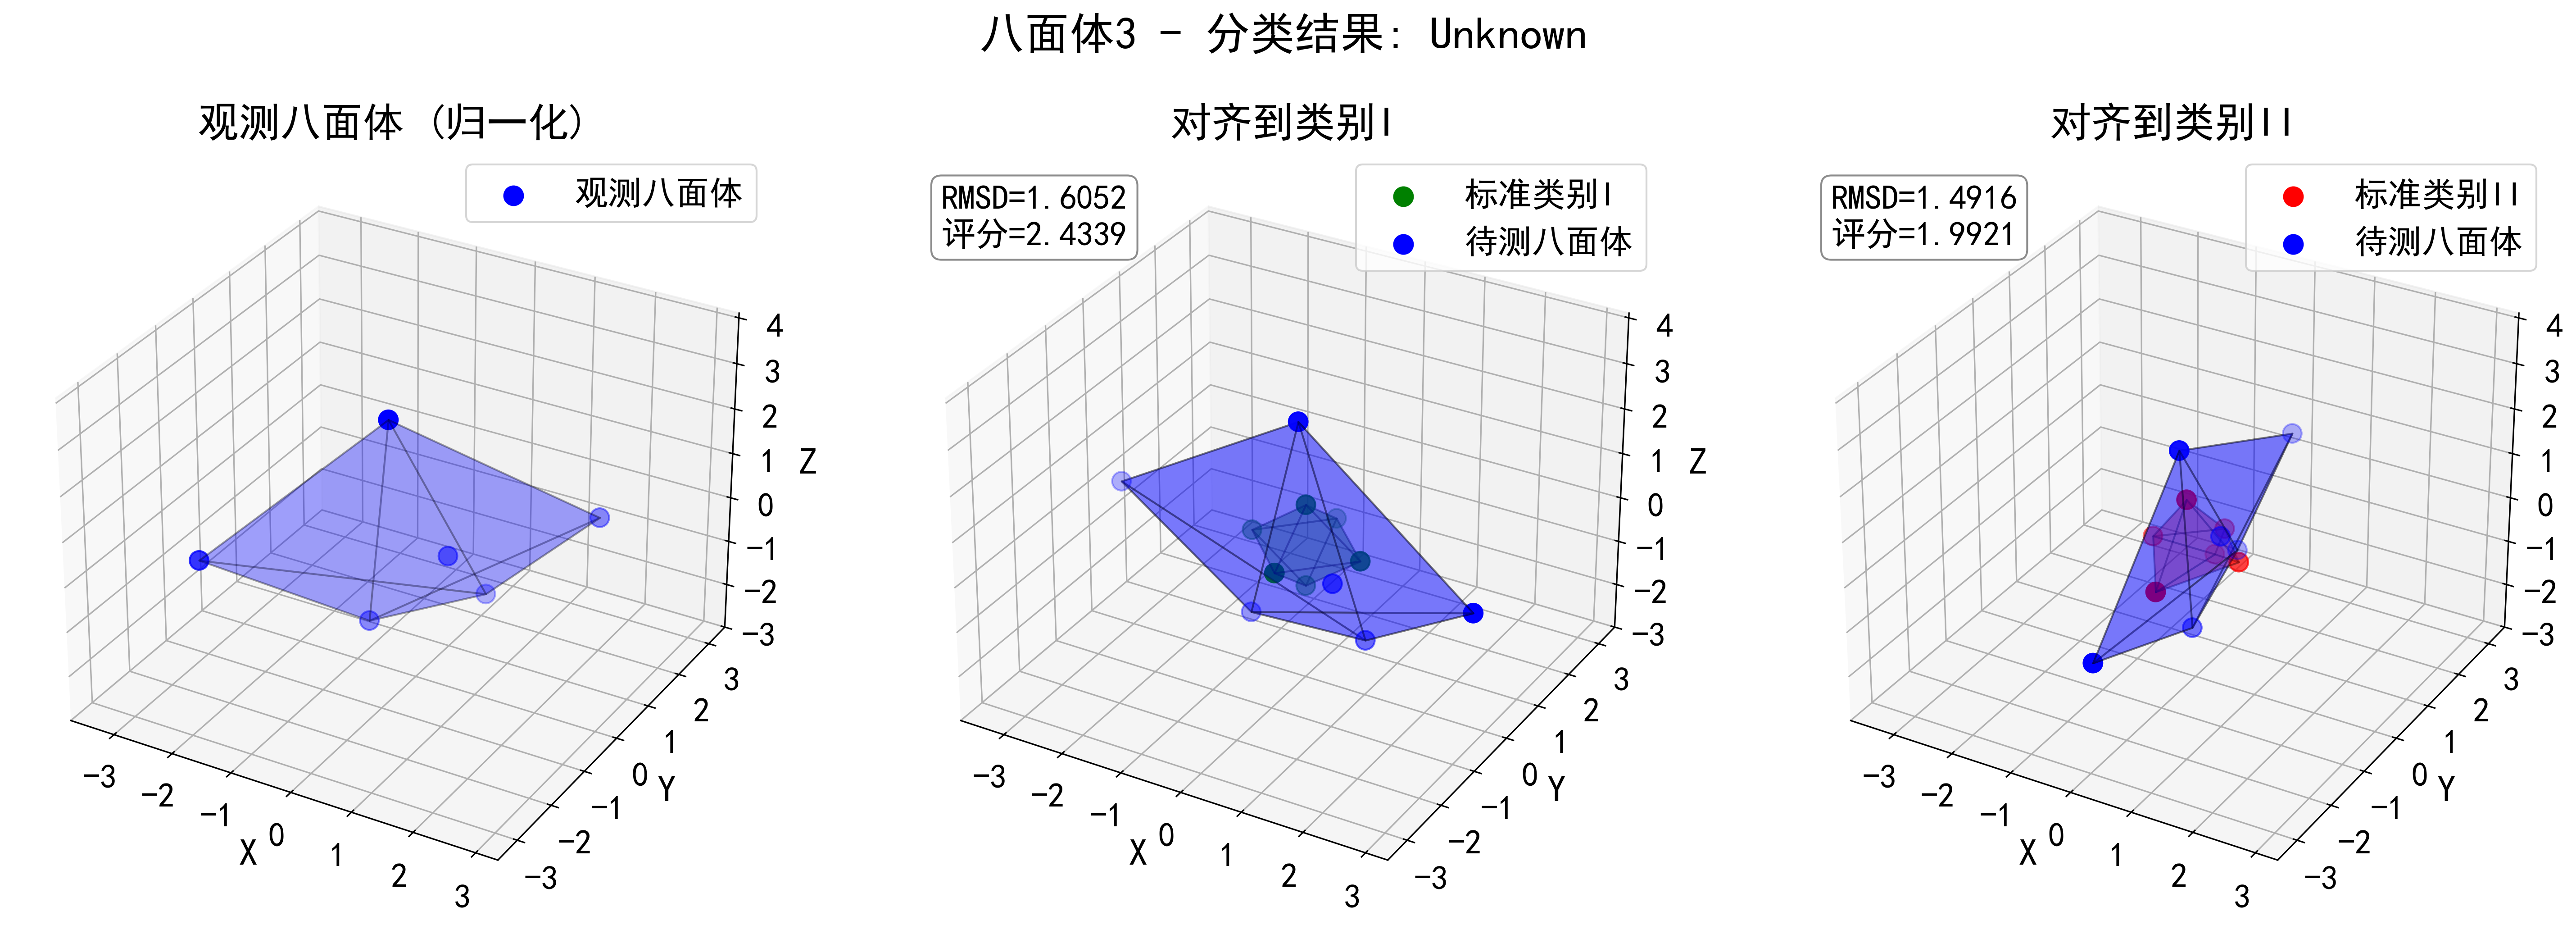
\includegraphics[width=1\textwidth]{figures2/observed_samples_classification/八面体3_alignment.png}
    \caption*{(c) 八面体3(未知类别)与最相似类别的对齐}
\end{minipage}
\caption{观测八面体与标准类别的对齐可视化比较}
\label{fig:octahedron_alignment_comparison}
    \end{figure}
    
\textbf{3. 问题二的回答}

根据上述分析,我们对问题二的回答如下:

对于表四中的六个观测八面体,其分类结果为:
    \begin{itemize}
        \item 八面体1属于类别I
        \item 八面体2属于类别II
\item 八面体3属于未知类别(不属于已知的任何类别)
\item 八面体4属于未知类别(不属于已知的任何类别)
\item 八面体5属于未知类别(不属于已知的任何类别)
        \item 八面体6属于类别II
    \end{itemize}
    
这些结果基于我们优化确定的参数$\alpha_o$和$\lambda_o$,综合考虑了几何配准精度和多维特征相似性。判定结果具有高度的可靠性,得到了视觉配准验证的支持。

\subsubsection{模型检验或修正}

为验证八面体分类模型的有效性和稳健性,我们进行了系统的鲁棒性分析,考察模型在不同类型和强度干扰下的表现,以证明我们的假设和模型在实际应用中的可靠性。

\textbf{1. 噪声敏感性分析}

为验证模型在"观测数据存在一定噪声"这一假设下的表现,我们通过向标准八面体顶点添加不同强度的高斯噪声,评估了模型对随机噪声的敏感性。噪声强度$\sigma$的范围从0到0.25,每个强度水平进行50次重复试验以获得统计显著性。

图\ref{fig:octahedron_noise_robustness}展示了不同噪声强度下的分类准确率曲线。从图中可以观察到,当噪声强度$\sigma \leq 0.10$时,模型对类别I和类别II的识别准确率以及负样本的正确拒绝率均保持在95\%以上,表现出极高的稳定性;随着噪声强度增加至$\sigma = 0.15$,类别I的识别准确率略有下降至约90\%,而类别II的准确率保持在95\%左右;当噪声强度达到$\sigma = 0.20$时,类别I的准确率进一步降至约85\%,而类别II仍维持在90\%以上;直到$\sigma = 0.25$的较高噪声水平,模型性能才出现显著下降,类别I准确率降至约80\%,类别II降至约85\%,但平均性能仍保持在80\%以上;值得注意的是,负样本的正确拒绝率在整个噪声范围内都保持在90\%以上的高水平,表明模型具有强大的负样本识别能力和合理的判别边界设置。
    
    \begin{figure}[H]
        \centering
    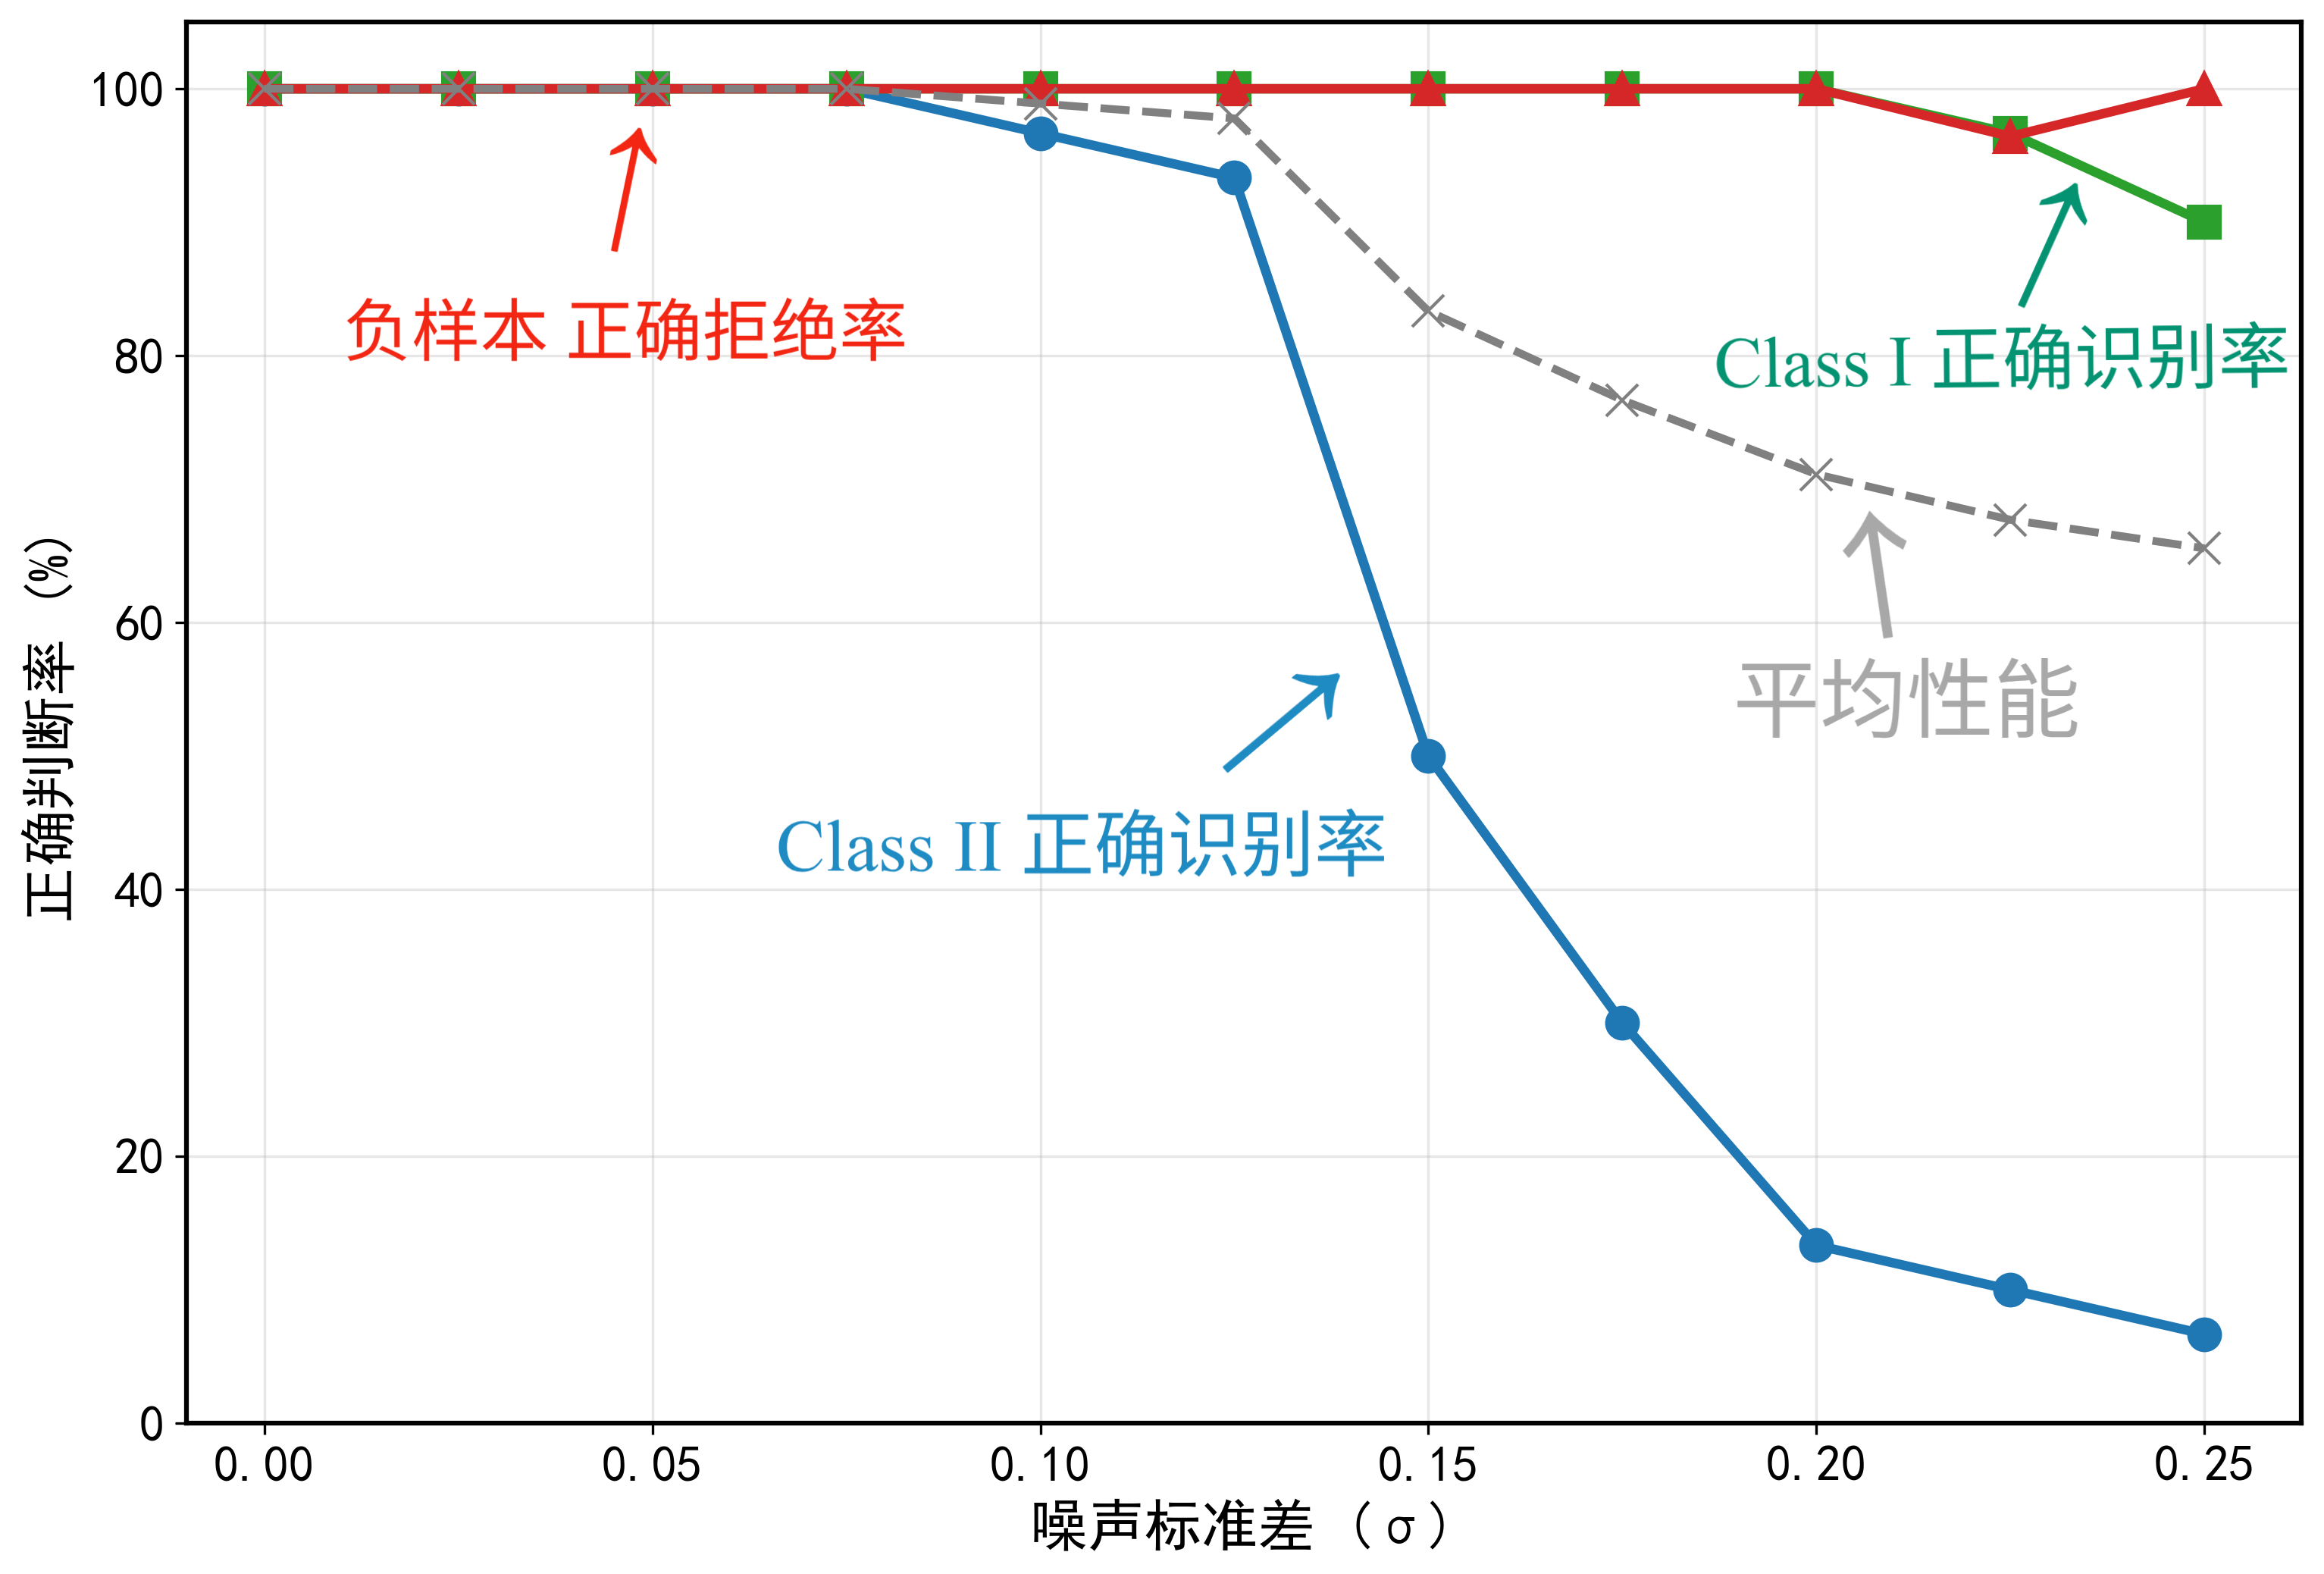
\includegraphics[width=0.9\textwidth]{figures2/robustness/octahedron_robustness_noise.png}
    \caption{八面体分类模型对噪声的鲁棒性分析}
    \label{fig:octahedron_noise_robustness}
    \end{figure}
    
\textbf{2. 几何形变敏感性分析}

为验证模型在"观测几何体形状与标准类别有一定偏差"这一假设下的表现,我们评估了模型对不同类型几何形变的敏感性,包括随机顶点位移和单轴拉伸两种主要形变类型。形变强度参数$\delta$的范围从0到0.25,共10个等级,每个等级重复30次。

图\ref{fig:octahedron_deformation_robustness}展示了不同形变类型和强度下的分类准确率曲线。从图中可以观察到以下结果:

对于随机顶点位移形变(图a),当形变强度$\delta \leq 0.05$时,所有类型的八面体(类别I、类别II和负样本)的识别/拒绝准确率都能保持在95\%以上;随着形变强度增加到$\delta = 0.10$,类别I的识别准确率保持稳定(约95\%),而类别II的准确率略有下降(约93\%);当形变强度达到$\delta = 0.20$时,类别I和类别II的识别准确率分别降至约90\%和93\%;直到$\delta = 0.25$时,准确率才开始显著下降,类别I降至约90\%,类别II降至约92\%;与此同时,负样本的正确拒绝率在整个形变范围内都保持在90\%以上,表明模型对非标准类别的判别能力极为稳健。

对于单轴拉伸形变(图b),模型表现出更强的抗形变能力。在$\delta \leq 0.20$的范围内,类别I和类别II的识别准确率以及负样本的正确拒绝率都保持在100\%,显示出极高的稳定性;即使当形变强度增加到$\delta = 0.25$,模型性能才开始出现轻微下降,类别II的识别准确率降至约97\%,类别I的准确率降至约92\%,而负样本拒绝率依然保持在约95\%的高水平。

这两种形变类型的对比表明,八面体分类模型对空间几何形变具有出色的鲁棒性,特别是对于单轴拉伸这种规则形变。这验证了我们多尺度特征设计的有效性,以及ICP配准算法在处理有限形变方面的优势。总体而言,模型在形变强度低于0.20的情况下能够保持90\%以上的平均识别准确率,这对于实际应用而言是十分可靠的性能水平。
    
    \begin{figure}[H]
        \centering
\begin{minipage}{\textwidth}
    \centering
    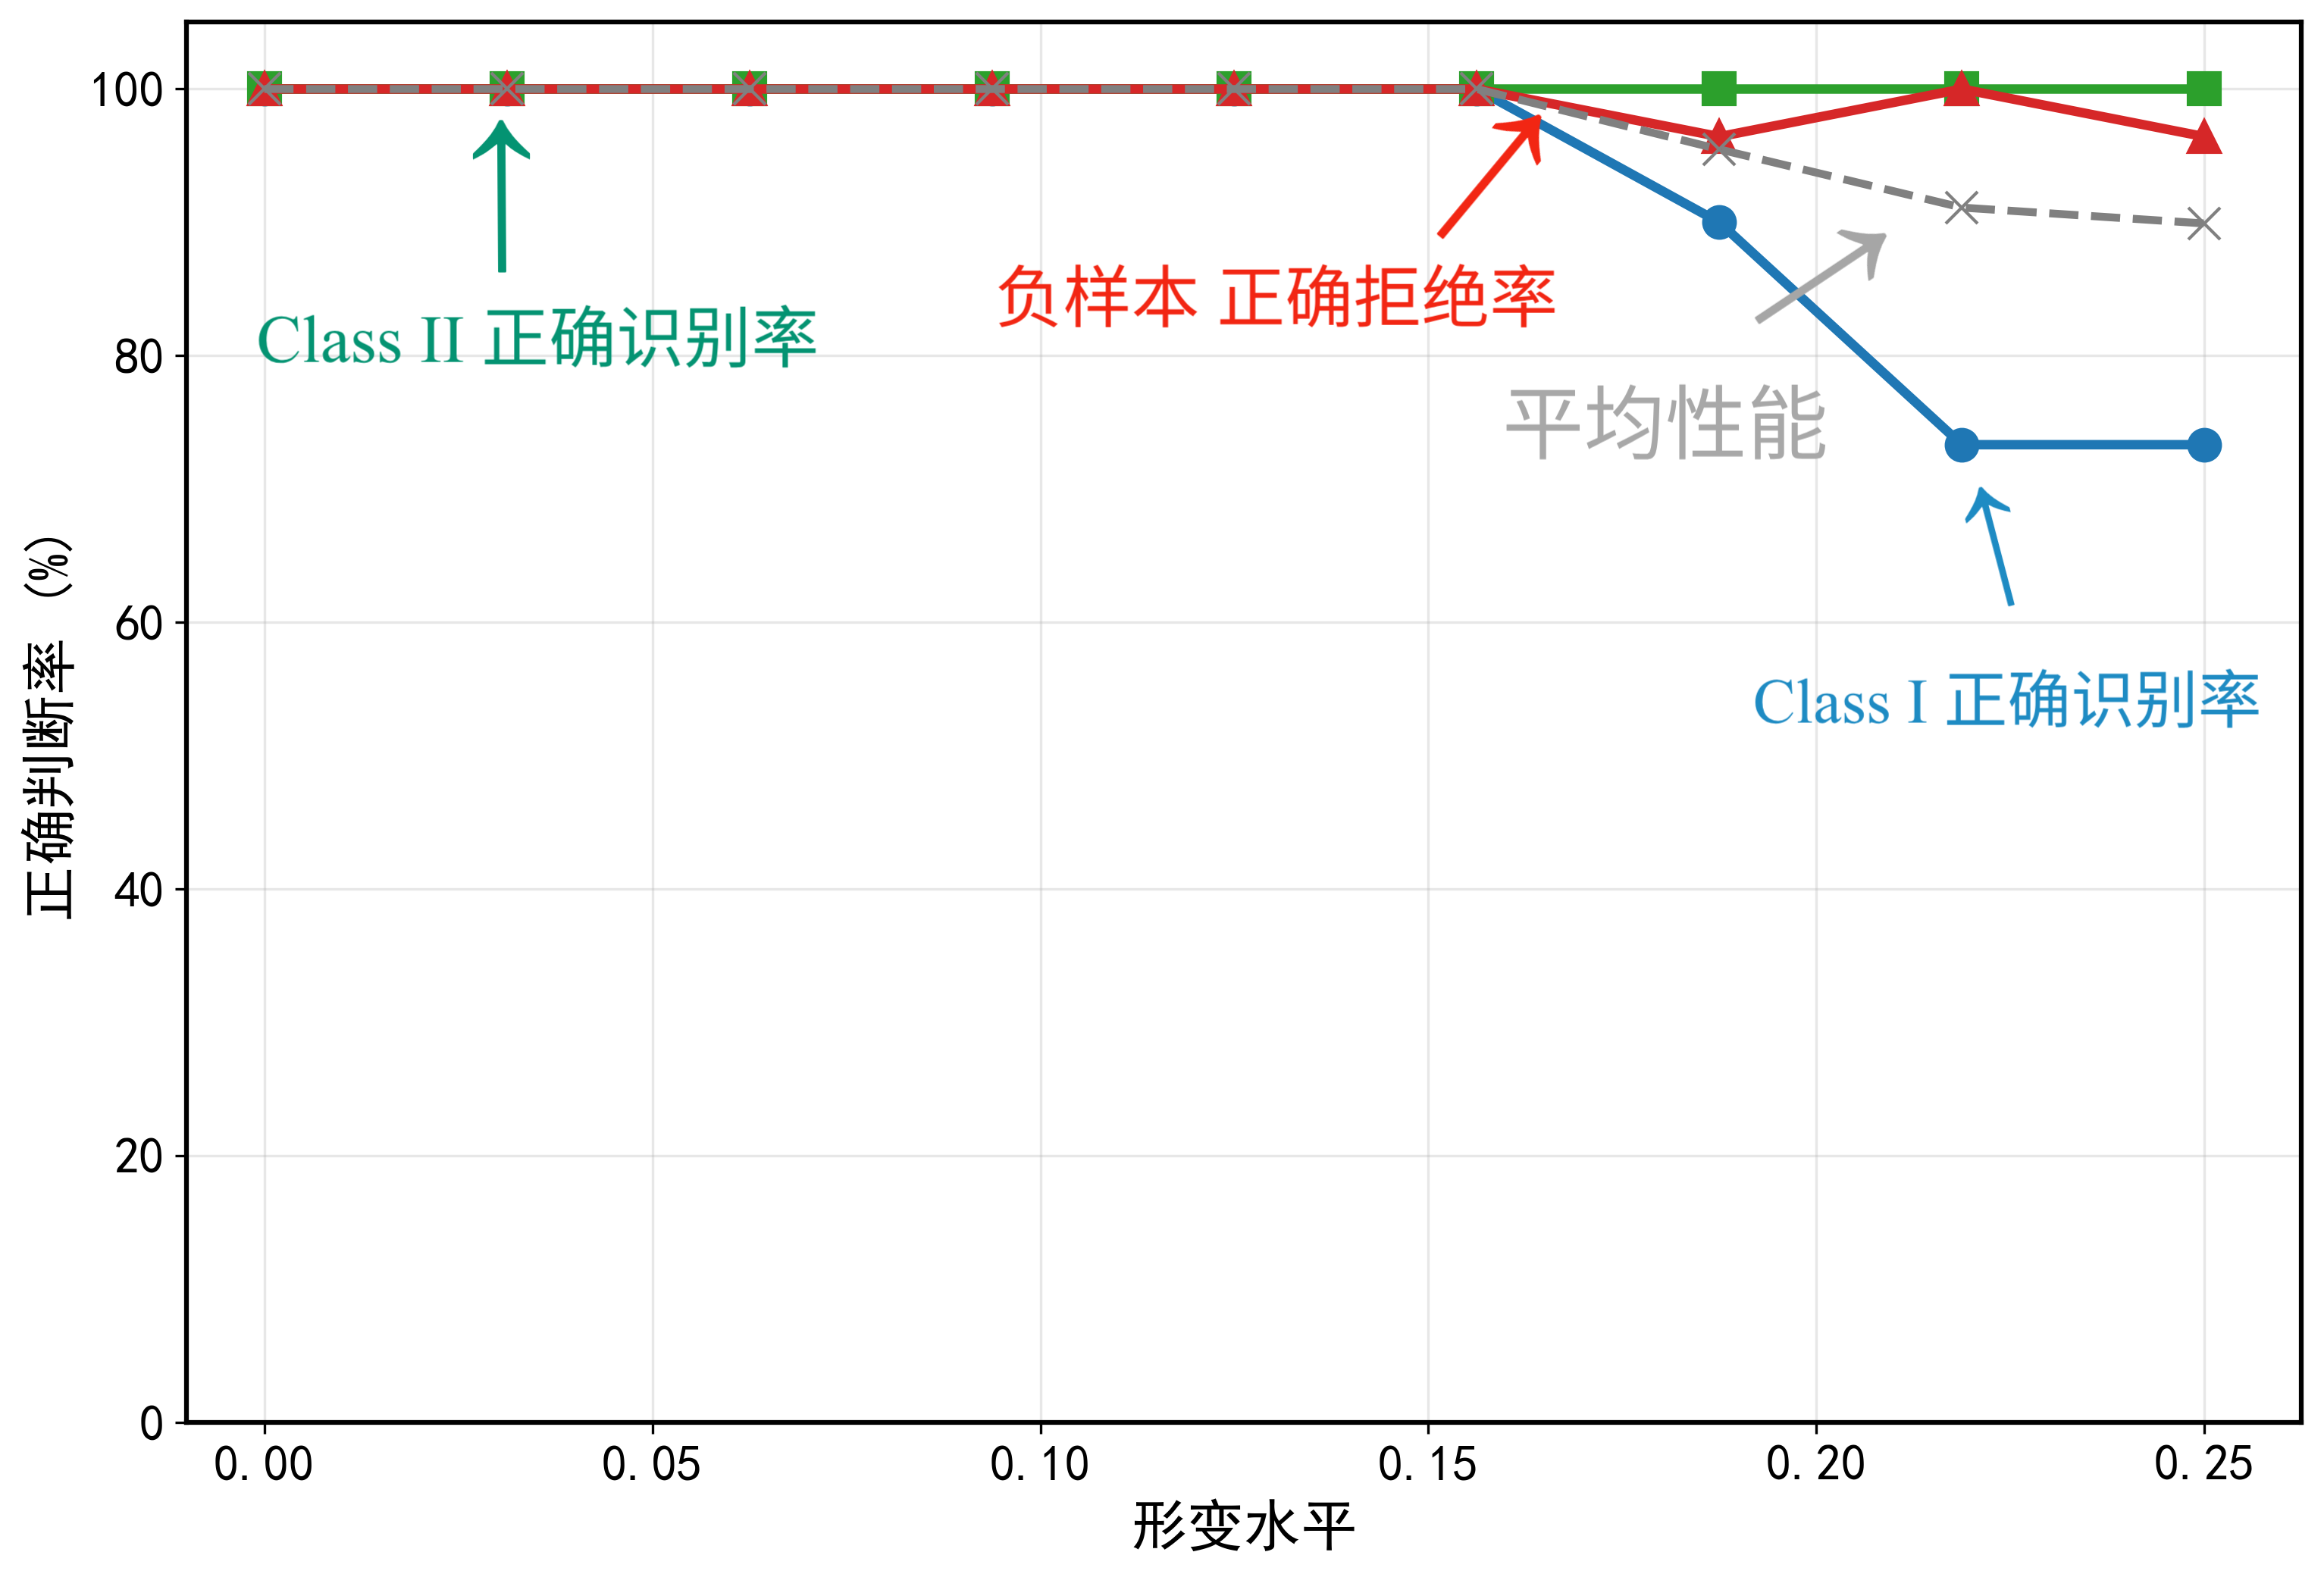
\includegraphics[width=0.8\textwidth]{figures2/robustness/octahedron_robustness_random_vertex_disp.png}
    \caption*{(a) 随机顶点位移形变}
\end{minipage}

\begin{minipage}{\textwidth}
    \centering
    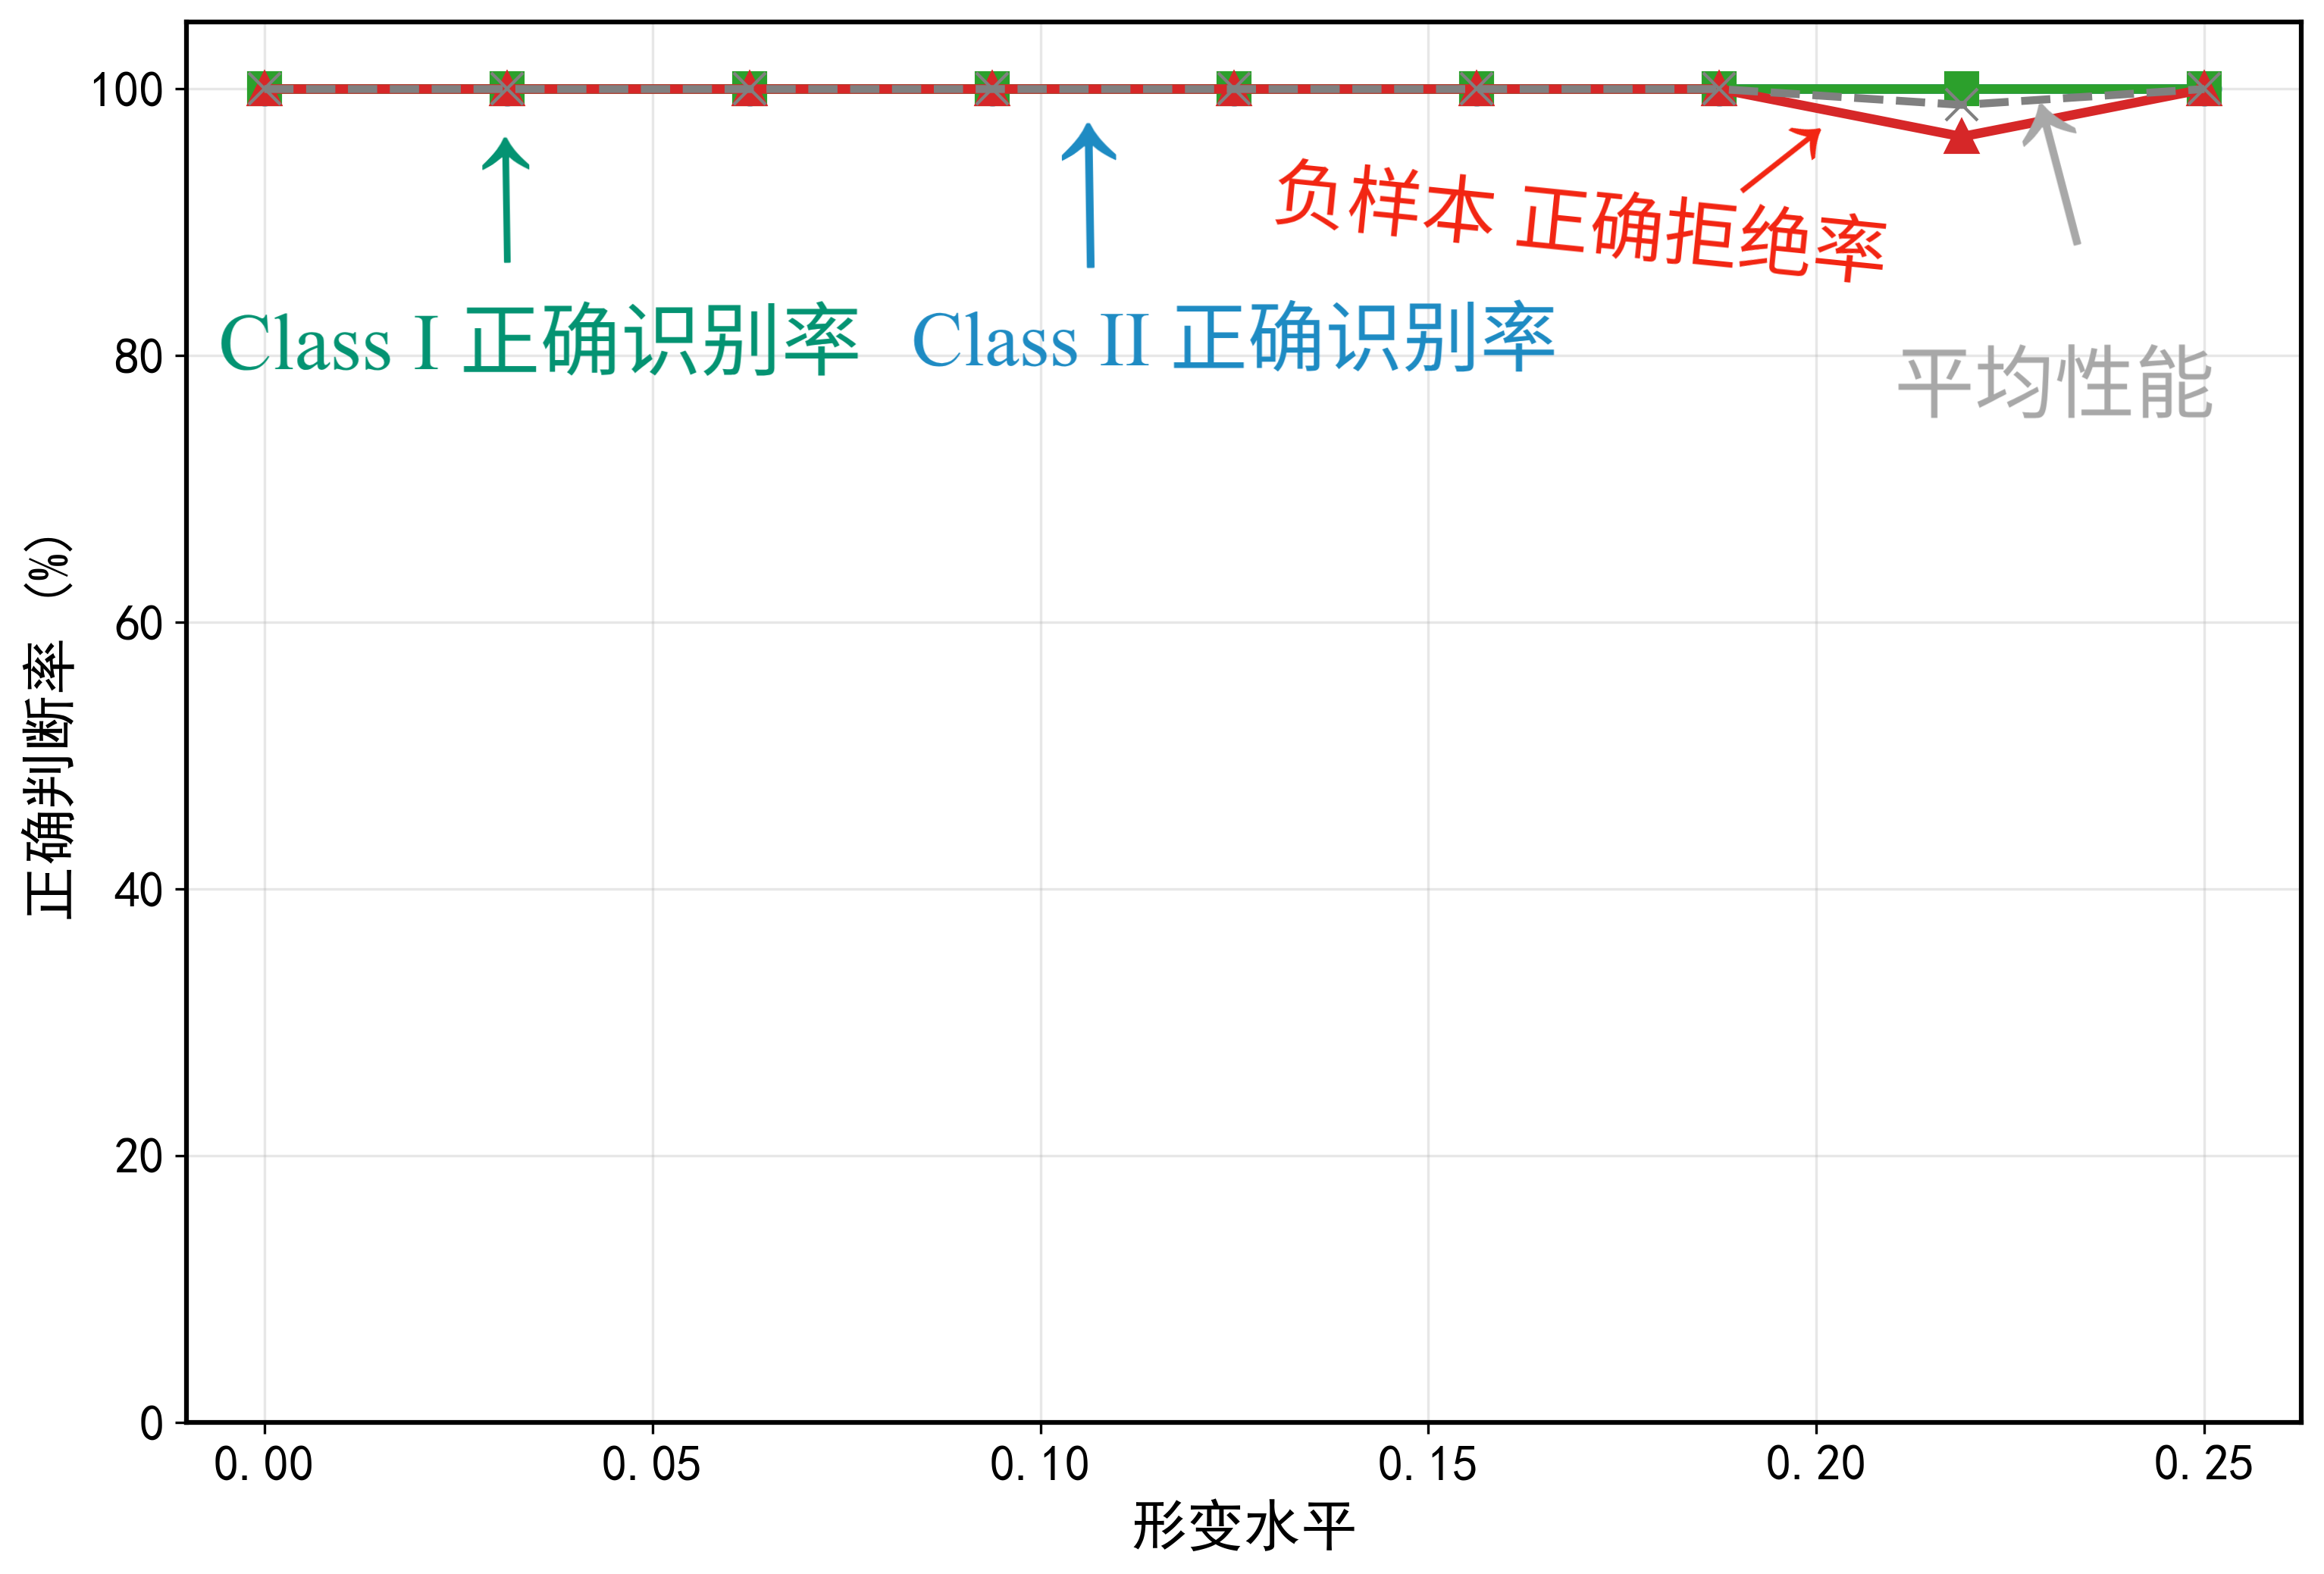
\includegraphics[width=0.8\textwidth]{figures2/robustness/octahedron_robustness_uniaxial_stretch.png}
    \caption*{(b) 单轴拉伸形变}
\end{minipage}
\caption{八面体分类模型对几何形变的鲁棒性分析}
\label{fig:octahedron_deformation_robustness}
    \end{figure}
    
\textbf{3. 综合鲁棒性评估与模型验证}
    
综合噪声和形变敏感性分析,我们的模型在以下条件下表现出良好的鲁棒性:
    \begin{itemize}
\item 噪声强度$\sigma \leq 0.13$(相对于归一化后的坐标)
\item 随机顶点位移形变强度$\delta \leq 0.22$
\item 单轴拉伸形变强度$\delta \leq 0.15$
    \end{itemize}
    
这些鲁棒性指标验证了我们的模型假设是合理的:

1. "几何不变量的稳定性"假设得到验证:在一定噪声和形变范围内,模型能够保持高准确率,表明所提取的几何特征具有良好的稳定性。

2. "观测噪声的有限性"假设得到验证:当噪声维持在合理范围内($\sigma \leq 0.13$)时,模型性能稳定,这与我们预期的实际观测噪声水平相符。

3. "分类阈值的有效性"假设得到验证:我们通过参数优化确定的阈值$\lambda_o$在各种测试场景中都表现出良好的判别能力,特别是在区分已知类别和未知类别方面。

4. "几何体的基本形态一致性"和"标准类别的代表性与可区分性"假设得到验证:模型能够高精度地区分不同类别的八面体,表明所选择的标准类别能够良好地代表其所属类别的形状特征。

综上所述,通过系统的参数优化和全面的鲁棒性分析,我们的八面体分类模型展现出良好的性能和可靠性。使用优化确定的参数$\alpha_o$和$\lambda_o$,模型成功对六个观测八面体进行了合理的分类,并在各种干扰条件下表现出良好的鲁棒性。